% Printing: http://www.pinders.uk.com/
% keyword ``report'' indicates positions to be changed
% vigra, cv1: part of ubuntu
% create keyword index
% bibliography by topic
% Cite "The Ruby Way?"


% wine,wrc,keyjnote
% ruby,irb,fxri,
% msys,mingw,
% boost,openexr,
% narray,
% qt4,qt4-ruby,
% imagemagick,rmagick,
% nsis,naturaldocs,
% cmu1394,directshow,dxva,mediaplayer,openexr,fftw3,narray

% ./configure --disable-shared
% ./configure --prefix=/MinGW

% detex
% PhD style file? !!!
\documentclass[a4paper,12pt]{book}

%\newif\ifpdf
%\ifx\pdfoutput\undefined
%\pdffalse                    % latex (print form)
%\else
%\pdfoutput=1                 % pdflatex (electronic form)
%\pdftrue
%\fi

% \usepackage{avantgar}   % Avantgarde
% \usepackage{bookman}    % Bookman
% \usepackage{chancery}   % Zapf Chancery, \textit only
% \usepackage{charter}    % Charter
% \usepackage{courier}    % Courier, \texttt only
% \usepackage{helvetic}   % Helvetica, \textsf only
% \usepackage{newcent}    % New Century Schoolbook
% \usepackage{palatino}   % Palatino
% \usepackage{times}      % Times
% \usepackage{utopia}     % Utopia
\usepackage{palatino}
\usepackage[utf8]{inputenc}
% \usepackage[latin1]{inputenc}
% \usepackage{ucs}
\newcommand{\thetitle}{Machine vision methods for microscopes and micromanipulation} % micromanipulation and microrobotics and microscopes
% Machine vision in the micro- and nano-environment
\newcommand{\shu}{Sheffield Hallam University}
\newcommand{\theauthor}{\href{http://www.multimap.com/map/browse.cgi?pc=S62UE}{Jan Wedekind}}
\newcommand{\mmvl}{Microsystems \& Machine Vision Laboratory}

% \newcommand{\narray}{\href{...}{NArray}}

% \usepackage[left=1cm,top=2cm,right=1cm,bottom=2cm,nohead,nofoot]{geometry}
% \usepackage[left=1.5cm,top=3cm,right=1.5cm,bottom=2cm]{geometry}

% use pseudo-code in main text !!!
% fully number equations, tables, and algorithms !!!

% questions from Bala (mock viva)
% How does limited depth of field between TEM/optical microscope compare
% What's the difference between depth of field and depth of focus?
% * dof: specimen can move without image appearing to lose focus
% * dim: the extent of the region of the image plane in which the image appears
%        sharp
% Simultaneuous estimation of blur PSF and restored image. You+Kaveh
% Methods of blind restoration of degraded images
% You use ``machine vision'' and ``computer vision'' interchangeably - explain
% What windowing fucntion? triangular/haming, why?
% How does non-linearity or sensitivity of camera systems affect this. Has
% camera been modelled?
% How is the NA reduced in the TEM? What is the mechanism in the TEM that
% allows this?
% Explain ``approximate'' shift invariant
% Explain expected original contributions!
% Statistics (object recognition performance).
% Use other images (instead of astronaut)

% Chris Care
% Don't elaborate on state-of-the-art not relevant to the final work!
% Content should lead up to final work.
% achieve publications (Journal) related to PhD to confirm novel contribution
% PhD and project have separate requirements
% Work on applications to microscopy (joint applications).

% \ifpdf
\usepackage[pdftex,final]{graphicx}
\DeclareGraphicsExtensions{.jpg,.pdf,.png}
% \else
% \usepackage[final]{graphicx}
% \DeclareGraphicsExtensions{.eps}
% \fi

\usepackage[british,UKenglish]{babel}
\usepackage[ruled]{algorithm2e}
\usepackage{amsfonts}
\usepackage{amsmath}
\usepackage{amsthm}
\usepackage{amssymb}
\usepackage{booktabs}
\usepackage{array}
\usepackage{calc}
\usepackage{units}
\usepackage[pdftex]{thumbpdf}
\usepackage{hyperref}
\usepackage{trfsigns}
\usepackage{txfonts}
\usepackage{verbatim}
\usepackage{units}

% \ifpdf
\pdfcompresslevel=9
\hypersetup{
   pdftitle      = {\thetitle},
   pdfsubject    = {PhD at \shu},
   pdfauthor     = {\theauthor},
   pdfkeywords   = {computer vision,machine vision,microscopy,micromanipulation,microassembly},
   pdfcreator    = {pdflatex},
   pdfproducer   = {LaTeX with several packages},
   bookmarksopen = true,
   bookmarksnumbered = true
}
% \fi

% \theoremstyle{definitions}
% \newtheorem{defn}{Definition}[section]

\begin{document}

\begin{titlepage}
  \noindent
  \begin{minipage}[c]{1.0cm}
    \resizebox*{\textwidth}{!}{
\includegraphics{shulogo}}
  \end{minipage}
  \begin{minipage}[c]{\linewidth minus 1.0cm}
    \begin{textrm}
      \shu\\
      \textbf{\mmvl\ (MMVL)}
    \end{textrm}
  \end{minipage}
  \vfill\noindent
  {\huge
    PhD thesis
    \bigskip\\
    \textbf{\thetitle}}
  \vfill\noindent
  \begin{large}\noindent
    \begin{tabular}{ll}
      Author      & Cand. PhD \theauthor\\
      &\\
      Supervisor  & Dr. Balasundram Amavasai \\
      &\\
      Period of time & 1.5.2005 -- 31.12.2008\\
    \end{tabular}
  \end{large}
\end{titlepage}

% Abstract?
\tableofcontents

\chapter{Introduction}
As the fields of micro- and nano-technology mature, there is going to be an
increased need for industrial tools that \emph{enable automated precision
assembly of micro-scale components}. The feedback mechanism in a future
micro-factory will likely require computer vision for feedback control.

Today optical microscopes, SEM\footnote{scanning electron microscopes}, and
TEM\footnote{transmission electron microscopes} are equipped with digital
cameras. Positioning of specimen and tool can be motorised
and controlled. Using real-time analysis of optical or electron/ion images
it could be possible to assist the operator of the microscope by providing
automatic positioning and alignment. Figure \ref{fig:jeol} shows the
controls of a TEM.
\begin{figure}[htbp]
   \begin{center}
     \resizebox{\textwidth}{!}{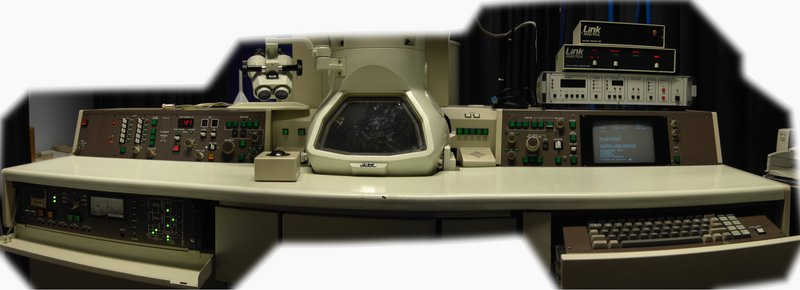
\includegraphics{jeol}}\\
     \caption{JEOL 3010 TEM at Sheffield University, Sorby Centre\label{fig:jeol}}
   \end{center}
\end{figure}
While solutions of this kind are conceivable, the realisation often fails due
to lack of integration of the different system components. Furthermore
the software for operating the microscope usually is proprietary and
does not give the necessary scope for development. In context of this work
a freely modifiable software platform is provided which offers integration
of a set of standardised system components. This platform then allows one to
% don't use ``allows to'' !!!
develop and test novel machine vision methods for the micro- and
nano-environment.

A literature review has been conducted to determine the state-of-the-art in
computer vision algorithms in general, and specifically to the field of
micro- and nano-imaging. The hardware architecture and the requirements for
integration were identified and specified. An
extension for the dynamically typed scripting language called
Ruby\footnote{\url{http://www.ruby-lang.org/}} is being developed to
serve as a basis for the final machine vision system. % Why Ruby? !!!
Currently this
Ruby extension offers file-I/O for images and videos, operator-based image
manipulations, image acquisition from IIDC/DCAM-compliant cameras and
Video-for-Linux devices, accelerated display using OpenGL or XVideo,
linear shift invariant filters, and high dynamic range imaging. The software
which has been developed so far can serve as a basis for developing a highly
customisable machine-vision-based control system with a graphical user
interface.

Limited depth of field dictates the choice of the
machine-vision algorithms employed in machine vision for TEM and optical
microscopes. In contrast to natural macro-scale images and SEM images where
the depth of field is virtually unlimited, the images generated by a TEM or
an optical microscope exhibit a very narrow depth of field. Furthermore the
projection of the object on the camera surface in an SEM as well as TEM and
optical microscopes is very close to an orthogonal projection. Scale changes
due to distance variation are thus very small. Hence many machine vision
algorithms developed for the macro environment are not applicable.

Currently the suitability of the dual-tree complex wavelet transform as
a means of extracting features which are, to some extent, invariant to focal
blurring is being investigated. As future work a robust object-recognition and
tracking algorithm for images with low depth of field is proposed. This can
be applied as a feedback-mechanism for automated micro- and
nano-manipulators. Thus this research seeks to achieve novel results in
machine vision and/or signal processing in the development and application of
computer vision methods to the micro- and nano-environment.

\chapter{Machine vision in microscopy}
Machine vision is a broad field and in many cases there are several
independent approaches to solve a particular problem. Also it is often
difficult to preconceive which approach will yield the best results.
For obvious reasons the machine vision software can only be tested in
a particular environment, after the hardware platform to run it on is
sufficiently developed. Experience shows that - since hardware and software
developers in a project often get to start and finish at the same time -
it is important to preserve the agility of the software to be able to
implement necessary changes at the end of a project. This
chapter gives an overview of the techniques considered for machine vision
in general and under the microscope. One or more of which may be used later on
within the context of this PhD and this research project.
% not known while writing this report

\section{State of the art}
A computer vision systems for object recognition and tracking usually
has a pipeline architecture as shown in figure \ref{fig:overview}.
\begin{figure}[htbp]
   \begin{center}
     \resizebox{\textwidth}{!}{
\includegraphics{overview}}\\
     \caption{Overview of a typical machine vision system\label{fig:overview}}
   \end{center}
\end{figure}
Some sub-systems may be missing but the sequence to process the sensor data
(here: a camera image) and recognise the objects usually consists of the
steps shown in table \ref{tbl:steps}.
\begin{table}[htbp]
  \begin{center}
    \caption{Processing steps performed by a typical machine vision
      systems\label{tbl:steps}} % explain !!!
    \begin{tabular}{ll}\toprule
      {\bf preprocessing}              & \parbox[t]{.6\textwidth}{basic operations such as filtering, thresholding, morphology and the like are applied to the image}\\
      {\bf key-point localisation} & \parbox[t]{.6\textwidth}{a feature extraction method defines feature locations in the image}\\
      {\bf feature description}     & \parbox[t]{.6\textwidth}{the descriptors for the local feature context are computed}\\
      {\bf recognition/tracking}    & \parbox[t]{.6\textwidth}{the features are used to recognise and track known objects in the scene}\\\bottomrule
    \end{tabular}
  \end{center}
\end{table}
There is a large resource of machine vision algorithms for recognising and
tracking objects. In the area of microscopy however
much of the current work focuses on analysing images and understanding the
image formation process to improve optical tomography.
There is only limited work on recognising and tracking micro-objects
and the degree of automation in microscopy leaves a lot to be desired. In the
next two sections a few algorithms which are particularly useful to the
micro-environment are presented.

\section{2-D recognition}\label{cha:2drecognition}
Often objects in microscopy are planar. In this case traditional
algorithms for recognition with two or three degrees of freedom
(x-, y-translation, and rotation) can be sufficient.
\cite{RefWorks:58}
presents an implementation of the geometric hashing algorithm using colour
segmentation for feature extraction to make the system stable against changing
illumination conditions.

One basic algorithm for 2-D recognition  is to use phase correlation. It can be
used to determine the position of a certain pattern in an
image\cite{RefWorks:432}.
Let $g\in\mathbb{Z}^2\to\mathbb{R}$ be a two-dimensional discrete function of
limited support representing an image. % explain !!!
Furthermore let $f$ be a shifted version of this image defined by
\begin{equation}\label{equ:shift}
  f(\vec{x})\coloneqq g(\vec{x}-\vec{\tau})
\end{equation}
Using $\delta_{\vec{\tau}}(\vec{x})\coloneqq\delta(\vec{x}-\vec{\tau})$
where $\delta$ is the Dirac distribution
\begin{equation*}
  \delta(\vec{x})\coloneqq\left\{\begin{array}{ll}
      \infty & \mathrm{for\ }\vec{x}=\vec{0}\\
      0 & \mathrm{otherwise}
    \end{array}\right.
\end{equation*}
equation \ref{equ:shift} can also be written as a convolution
$f=g\,\otimes\delta_{\vec{\tau}}$. In Fourier space the convolution
becomes a multiplication
\begin{equation*} % explain fourier-transform symbol !!!
  f=g\,\otimes\delta_{\vec{\tau}}\ \fourier\ F=G\cdot\Delta_{\vec{\tau}}
\end{equation*}
where $\Delta_{\vec{\tau}}(\vec{\omega})=\mathcal{F}\{\delta_{\vec{\tau}}\}(\vec{\omega})=e^{-<\vec{\omega},\vec{\tau}>\,\mathbf{i}}$.

If $f$ and $g$ are given and the shift vector $\vec{\tau}$ is not known,
it can be estimated by first computing the normalised product of $F$ and $G$ as
follows\cite{RefWorks:432}
% explain: conjugates, normalised, normalised cross correlation !!!
\begin{equation*}
R\coloneqq\frac{F\,G^{*}}{|F\,G^{*}|}
\end{equation*}
and then determining the maximum of the inverse Fourier transform of the result
\begin{equation*}
  \widehat{\vec{\tau}}=\mathop{\mathrm{argmax}}_{\vec{\tau}\in\mathbb{Z}^2}\big(r(\vec{\tau})\big)
  \mathrm{\ where\ }r=\mathcal{F}^{-1}\{R\}
\end{equation*}
% explain: selecting maximum, estimating translation/shift !!!
This algorithm can be used to align images as shown in figure \ref{fig:phasecorrelation}.
\begin{figure}[htbp]
   \begin{center}
     \resizebox{.6\textwidth}{!}{\includegraphics{phasecorrelation}}\\
     \caption{Aligning two images using phase
       correlation\label{fig:phasecorrelation}}
   \end{center}
\end{figure}
\cite{RefWorks:432} extends the phase correlation to not only provide
translation but rotation as well. % explain search process !!!
% Wiener filter?

The implementation of the algorithm in Ruby follows here
% \tiny   \small  \large  \huge  \scriptsize  \normalsize  \Large
% \Huge  \footnotesize   \LARGE
\begin{scriptsize}
  \verbatiminput{phasecorrelation.rb}
\end{scriptsize}
% MINIMAN?

2-D recognition is not necessarily limited to planar objects. Figure
\ref{fig:pipette} shows a microscope image of a pipette. The intersection
of the pipette with the focused plane has been detected using 2-D
recognition\footnote{\url{http://vision.eng.shu.ac.uk/mmvlwiki/index.php/Microscope_Vision_Software}}. % explain more? !!!
\begin{figure}[htbp]
   \begin{center}
     \resizebox{.6\textwidth}{!}{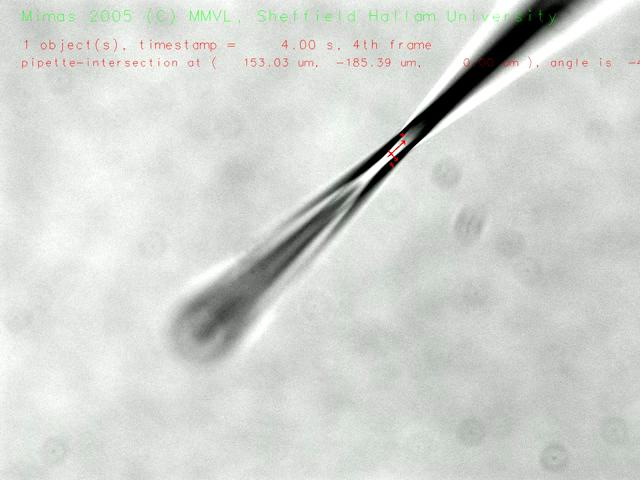
\includegraphics{pipette}}\\
     \caption{2-D recognition can be used to determine the intersection of a
       pipette with the focused plane\label{fig:pipette}}
   \end{center}
\end{figure}

\section{3-D recognition}
Methods for 3-D in the macro-environment usually cannot be applied to
microscopy images at all or at least need modification since the depth of
field is limited. However there are techniques in machine vision to deal with
or even exploit limited depth of field. In this section a couple of
state-of-the-art methods are presented which goes beyond simple 2-D
recognition.

\subsection{Autofocus}
Automatic adjustment of camera focus is a problem that occurs in digital still
cameras, which are essentially commodity devices. Autofocus usually is
performed by adjusting the focus drive, capturing an image, and computing a
sharpness measure in a loop. To find the maximum of the (unknown) sharpness
function in real-time (see figure \ref{fig:autofocus}).
\begin{figure}[htbp]
   \begin{center}
     \resizebox{.3\textwidth}{!}{
       \begin{picture}(0,0)
         \input{autofocus.pstex_t}
       \end{picture}
       \includegraphics{autofocus}}
     \caption{Typical characteristic of a sharpness
       measure\label{fig:autofocus}}
   \end{center}
\end{figure}
Often the sharpness measure is estimated by computing it only for a part of
the image or for a down-sampled version of the image
as shown in \cite{RefWorks:435}. Popular sharpness measures are the
maximum norm of the Sobel gradient and the local variance of the image.

If $g_z\in\mathbb{Z}^2\to\mathbb{R}$ is the image acquired with focal setting
$z$, the estimated optimal focal setting $\widehat{z}$ is
\begin{equation*}
  \widehat{z}=\displaystyle\mathop{\mathrm{argmax}}_{z}
  \sum_{x_1}\sum_{x_2} ||\mathrm{SOBEL}\{g_z\}(\vec{x})||_{\infty}
\end{equation*}
where $||\cdot||_{\infty}$ is the maximum norm. See appendix
\ref{cha:sobeledges} for a description of the Sobel operator.
% correct referencing of appendix !!!

There are more sophisticated sharpness measures. For example
\cite{RefWorks:436} shows how to compute a sharpness measure based on
moments which is largely independent of the image content. Since
sharpness measures rely on object textures which are not always present,
some digital still cameras use a separate optic with a LED to project a
pattern on the scene.

Autofocusing is also applied in microscopy. \cite{RefWorks:42} shows how
one can use an autofocusing algorithm for manipulating cells under a
microscope. While focal blurring is much more severe under optical microscopes,
the resulting reduced depth of field also allows for a more accurate
estimation of the micro-object's distance.

Approaches for 2-D recognition of objects can be extended to include depth
as shown in \cite{RefWorks:431}. Instead of comparing the scene with a single
2-D model of the micro-object, the scene is compared with a set of 2-D models
of the micro-object which is created from a focus stack. While this approach
allows one to recognise and track multiple micro-objects at different depth,
the micro-objects are only allowed to rotate around the optical axis of the
imaging microscope. Other rotations will lead to the system loosing track of
the micro-object. Figure \ref{fig:gripper} shows a micro-gripper being
recognised and tracked.
\begin{figure}[htbp]
   \begin{center}
     \resizebox{.4\textwidth}{!}{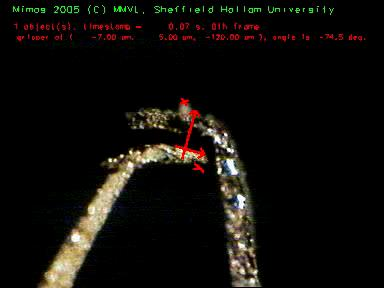
\includegraphics{gripper}}\\
     \caption{Estimating 2-D position and depth of a
       micro-gripper\cite{RefWorks:431}\label{fig:gripper}}
   \end{center}
\end{figure}

\subsection{Depth From Focus}
% explain ``is much more noticeable than'' !!!
The focal blur under optical microscopes usually is much more noticeable than
the focal blur encountered in macroscopic environments. Reducing the
aperture size or the numerical aperture will increase the depth of field.
However reducing the aperture size requires compensation by increasing the
illumination, exposure time, or camera sensivity. Reducing the numerical
aperture on the other hand leads to higher diffraction and thus reduces the
resolving power of the system.

While the limited depth of field can rule out 3-D reconstruction using
laser line projection, a sharpness measure can be used to estimate the
distance of an object. Furthermore it is possible to reconstruct surfaces up
to a certain resolution by using a local sharpness measure. If the microscope
allows one to project % explain !!!
a pattern on the object (as shown in figure \ref{fig:smallwheelg}) this can
improve the stability of the algorithm
\begin{figure}[htbp]
   \begin{center}
     \resizebox{.6\textwidth}{!}{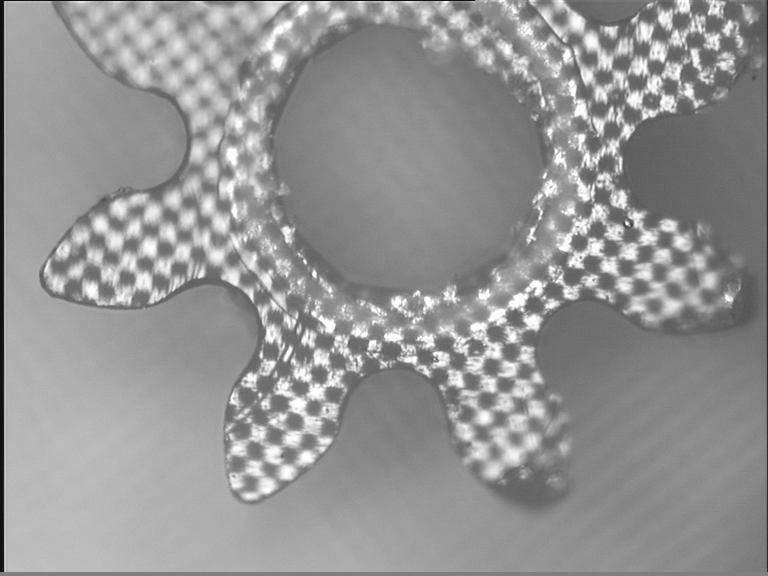
\includegraphics{smallwheelg_335}}\\
     \caption{Microscope image of a small cogwheel illuminated with a projected
       pattern\cite{RefWorks:437}\label{fig:smallwheelg}}
   \end{center}
\end{figure}

% point out that this work was done by me !!!
Equation \ref{equ:depthmap} shows how a depth map can be estimated by
searching the maximum of the sharpness measure if a focus stack
$\{g_z|z\in\{z_1,z_2,\ldots\}\}$ of microscope images with different
focal setting $z$ is given
\begin{equation}\label{equ:depthmap}
  \displaystyle D(\vec{x})\coloneqq\mathop{\mathrm{argmax}}_{z\in\{z_1,z_2,\ldots\}}\big(\mathrm{SOBEL}\{g_z\}(\vec{x})\big)
\end{equation}
The focus stack can be acquired by using a motorised stage to move
the micro-object away from the microscope step-wise (along the optical axis)
and taking a series of images. The resulting surface estimate can for example
be used in forensics to measure firing pin marks and characteristic grooves
caused by the barrel which can be used for classification\cite{RefWorks:130}.

\cite{RefWorks:57} shows how to create 3-D reconstructions of periodical
movements of MEMS\footnote{micro-electro-mechanical systems} by using
depth from focus and stroboscope illumination. The system can be used for
verifying MEMS prototypes.

The algorithm depends on local textures in the image. Since the quality of
the texture may vary within the image, taking a weighted average of
the result as in \cite{RefWorks:438} or using a multi-resolution approach
as in \cite{RefWorks:43} will greatly improve the estimate of the
micro-object's surface as shown in figure \ref{fig:smallwheel}.
A detailed discussion of this techniques is beyond the scope of this report.
\begin{figure}[htbp]
   \begin{center}
     \resizebox{.6\textwidth}{!}{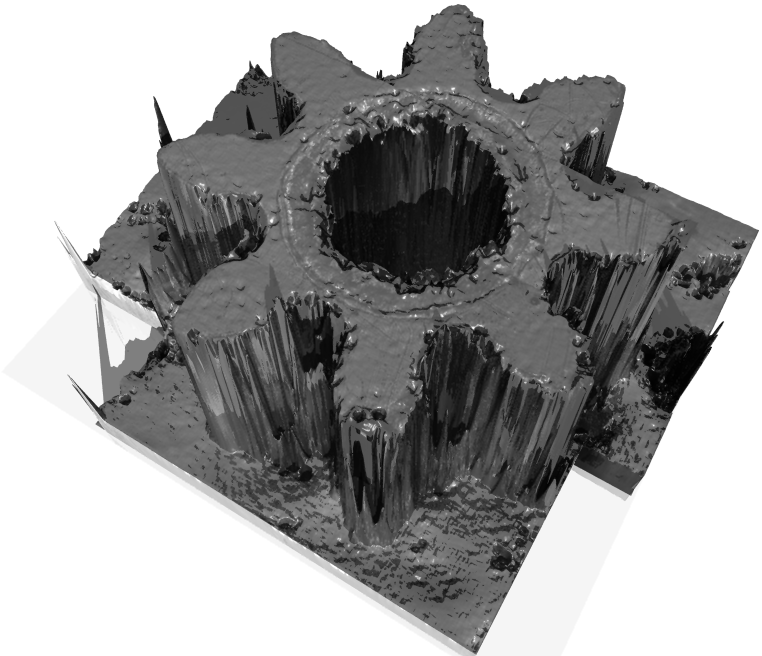
\includegraphics{smallwheel}}\\
     \caption{Surface of a small cogwheel (diameter \unit[0.6]{mm})
       reconstructed from three focus
       stacks\cite{RefWorks:437}\label{fig:smallwheel}}
   \end{center}
\end{figure}

Depth from focus typically requires acquisition and processing of more than
100 images and thus it is hard to do in real-time. However there is a strong
motivation to achieve this goal since acquisition of depth maps in 
real-time makes it possible to determine the depth of objects in real-time.
\cite{RefWorks:121} demonstrates a system consisting of a dynamic
focusing lens and a camera with a digital signal processor for performing
depth from focus in real-time. It is also possible to move the sensor
instead of the lens as shown in \cite{RefWorks:439}. So far this systems
are only used to determine the depth and shift of objects (\emph{i.e.} only
three degrees-of-freedom). However depth maps of sufficient quality would make
it possible to apply 3-D recognition using spin-images as shown in
\cite{RefWorks:433}. Such a system could provide pose-estimation for
micro-objects with six degrees-of-freedom.

\subsection{Depth From Defocus}
Depth from defocus attempts to estimate the depth of the object
from a focus set of only two images $i_1$ and $i_2$\cite{RefWorks:142}.
If the imaging system is calibrated, for a given depth $\alpha$ the focal blur
$h(\alpha)$ is known. Assuming the depth $\alpha$ of the scene is constant,
the two images $i_1$ and $i_2$ are related as follows
\begin{equation*}
  \begin{split}
    i_1&=g\otimes h(\alpha)\\
    i_2&=g\otimes h(1-\alpha)
  \end{split}
\end{equation*}
where $g$ is the focused image which could be acquired if the depth $\alpha$
would be known. The corresponding equation in Fourier becomes a multiplication
as shown below
\begin{equation*}
  \begin{split}
    I_1&=G\,H(\alpha)\\
    I_2&=G\,H(1-\alpha)
  \end{split}
\end{equation*}
Depth from defocus is based on the following term $M/P$ which changes with
the depth $\alpha$ but is independent of the image content $G$
\begin{equation*} % explain M and P before defining them !!!
  \cfrac{M}{P}\coloneqq\cfrac{I_1-I_2}{I_1+I_2}=\cfrac{H(\alpha)-H(1-\alpha)}{H(\alpha)+H(1-\alpha)}
\end{equation*}
According to \cite{RefWorks:142} this relation can be modelled in Fourier
space using $Q_M$, $Q_{P_1}$, and $Q_{P_2}$ as follows
($\beta$ is a non-linear monotonous function of $\alpha$)
\begin{equation*} % explain Q_M, ... !!! Use glossary? !!!
  Q_M\,M=\big(\beta(\alpha)\,Q_{P_1}+\beta^3(\alpha)\,Q_{P_2}\big)\,P+\epsilon
\end{equation*}
An optimal combination of $Q_M$, $Q_{P_1}$, $Q_{P_2}$ and $\beta$ can be
derived for a particular imaging system. In picture space the multiplications
become convolutions.
\begin{equation}\label{equ:defocus}
  q_m\otimes(i_1+i_2)=\big(\beta(\alpha)\,q_{p_1}+\beta^3(\alpha)\,q_{p_2}\big)\otimes (i_1-i_2)+\epsilon
\end{equation}
Note that if the filters $q_m$, $q_{p_1}$, and $q_{p_2}$ have been optimised
to have limited support in picture space, it is possible to estimate the depth
in a local region of the image. In this case it is possible to apply this
method even if the depth of the scene $\alpha$ is not constant, and one can
obtain depth maps using equation \ref{equ:defocus}.
Given two images $i_1$ and $i_2$ the depth can be estimated in real-time by
convolving $m$ and $p$ with the convolution filters $q_m$, $q_{p_1}$, and
$q_{p_2}$ and then estimating the value $\widehat{\alpha}$ which minimises
the error $\epsilon$.

Figure
\ref{fig:depthfromdefocus} shows the result obtained from a pair of
test images.
% explain :( !!!
\begin{figure}
   \begin{center}
     \begin{minipage}[c]{.3\textwidth}
       \resizebox{\textwidth}{!}{\includegraphics{defocus1}}
     \end{minipage}\&
     \begin{minipage}[c]{.3\textwidth}
       \resizebox{\textwidth}{!}{\includegraphics{defocus2}}
     \end{minipage}$\Rightarrow$
     \begin{minipage}[c]{.3\textwidth}
       \resizebox{\textwidth}{!}{\includegraphics{depthfromdefocus}}
     \end{minipage}
     \caption{Input images and depth map estimated with depth from
       defocus\label{fig:depthfromdefocus}}
   \end{center}
\end{figure}
However, apart from being difficult to implement, depth from defocus is highly
sensitive and imposes several constraints on the environment:
\begin{itemize}
\item focal blur must be small compared to the object size
\item all objects must reside between the two focused planes
\item the images must be aligned with high accuracy
\item the scene must be stationary
\item the image must not exhibit artefacts other than focal blurring
\item the algorithm heavily relies on object textures
\end{itemize}

Note that it may not be possible to use a projection pattern to introduce
local texture content, because usually the projection optic also has
its own focal blur and this will lead to different blur of projected patterns
and object textures.

\subsection{Disparity Estimation}
Depth estimation can also be done by applying a disparity estimator to
a set of stereo images. % explain disparity estimator !!!
\begin{itemize}
\item focal blur must be small compared to the object size and the disparity
  must be sufficient
\item stereo imaging usually requires calibration of the cameras
\item the algorithm relies on object textures
\end{itemize}

If no stereo-microscope is available, there is still the possibility of
stereo from motion. Since the disparity resulting from a lateral motion under
the microscope often is insufficient, the micro-object is rotated
instead\footnote{see \url{http://www.vcbio.science.ru.nl/en/image-gallery/3drendering/}}.

While disparity estimation itself is not an easy task, it is also not easy
to apply it to microscopic imaging. However its usefulness for object
recognition and tracking in the microscopic environment cannot be ruled out
entirely.
% mirror (EPFL)

\chapter{Proposed system}
The aim of the current work is to develop and integrate a system for
recognising and tracking objects in the micro-environment. % report is to early
To facilitate the research to be undertaken, a Ruby-extension called
\emph{HornetsEye} is under development to serve as a basis for implementing
and integrating machine vision algorithms. The current state of this work is
presented in this chapter. The library is released under the GPL license and
it is available for download at
\begin{itemize}
\item \url{http://www.wedesoft.demon.co.uk/hornetseye-api/}
\item \url{http://vision.eng.shu.ac.uk/mediawiki/index.php/Hornetseye}
\item \url{http://rubyforge.org/projects/hornetseye/}
\item \url{http://sourceforge.net/projects/hornetseye/}
\item \url{http://raa.ruby-lang.org/project/hornetseye/}
\end{itemize}

\section{Sensor input}
\subsection{Image acquisition}
The first step performed by a typical machine vision system (see fig.
\ref{fig:overview} previously) is to retrieve sensor input. In this report
images are represented as discrete, infinite, high dynamic range,
black-and-white functions (see table \ref{tbl:image}) if not stated
otherwise.
\begin{table}[htbp]
  \begin{center}
    \caption{Different types of images\label{tbl:image}} % explain !!!
    \begin{tabular}{ll}\toprule
      \parbox[t]{.35\textwidth}{discrete, finite, quantised, black-and-white function} &
      \parbox[t]{.55\textwidth}{$g\in\{0,1,\ldots,w-1\}\times\{0,1,\ldots,h-1\}\to\{0,1,\ldots,255\}$}\\
      \parbox[t]{.35\textwidth}{discrete, finite, high dynamic range, black-and-white function} &
      \parbox[t]{.55\textwidth}{$g\in\{0,1,\ldots,w-1\}\times\{0,1,\ldots,h-1\}\to\mathbb{R}$}\\
      \parbox[t]{.35\textwidth}{discrete, infinite, high dynamic range, black-and-white function} &
      \parbox[t]{.55\textwidth}{$g\in\mathbb{Z}^2\to\mathbb{R}$}\\
      \parbox[t]{.35\textwidth}{continuous, infinite, high dynamic range, black-and-white function} &
      \parbox[t]{.55\textwidth}{$g\in\mathbb{R}^2\to\mathbb{R}$}\\\midrule
      \parbox[t]{.35\textwidth}{discrete, finite, quantised, colour function} &
      \parbox[t]{.55\textwidth}{$\vec{c}\in\{0,1,\ldots,w-1\}\times\{0,1,\ldots,h-1\}\to\{0,1,\ldots,255\}^3$}\\
      \parbox[t]{.35\textwidth}{discrete, finite, high dynamic range, colour function} &
      \parbox[t]{.55\textwidth}{$\vec{c}\in\{0,1,\ldots,w-1\}\times\{0,1,\ldots,h-1\}\to\mathbb{R}^3$}\\
      \parbox[t]{.35\textwidth}{discrete, infinite, high dynamic range, colour function} &
      \parbox[t]{.55\textwidth}{$\vec{c}\in\mathbb{Z}^2\to\mathbb{R}^3$}\\
      \parbox[t]{.35\textwidth}{continuous, infinite, high dynamic range, colour function} &
      \parbox[t]{.55\textwidth}{$\vec{c}\in\mathbb{R}^2\to\mathbb{R}^3$}\\\bottomrule
    \end{tabular}
  \end{center}
\end{table}
This representation allows one to accurately model an image capturing device
with a grid of rectangular photosensitive cells without having to formally
threat the boundaries of the camera-chip. % explain !!!
There is no upper limit for
$g(\vec{x})$ which expresses the fact that there is no upper limit for
luminosity (see \cite{RefWorks:422} for a detailed introduction to high
dynamic range imaging). The range displayable on a low dynamic range device
(such as a monitor or a printout) is $\{0,1,\ldots,255\}$ for quantised
and $[0,1]$ for analog (non-quantised) images.

% The human response of the three channels is also non-linear !!!
Humans have trichromatic vision.
There are different colourspaces for representing trichromatic images.
Frequently the RGB (red-green-blue) colourspace is used with spectral
intensity maxima at 475 nm (blue), 510 nm (green), and 650 nm (red) wavelength
in the electromagnetic spectrum. These are not as generally believed the
sensitivity maxima of the human photosensitive cones, which are at 445 nm,
535 nm, and 570 nm\cite{RefWorks:440} (furthermore the photoreceptors for
black-and-white vision at night have their sensitivity maximum at 507 nm).
However as long as the sensitivity curves of the three colour channels of the
camera are more or less accurate linear combinations of the sensitivity curves
of the human visual cortex, it is possible to accurately reproduce the visual
impression perceived by the human visual cortex.
% http://www.psych.ndsu.nodak.edu/mccourt/Psy460/Color%20Vision/Color%20Vision.html

High dynamic range images are not displayed here since the file-format used
for this report does not support high dynamic range images.
Figure
\ref{fig:hdr} shows an image $g^\prime$ created using a high dynamic
range image $g$ of a scene with high contrast. The image was multiplied with
an exposure ramp ($g^\prime(\vec{x})=g(\vec{x})\,x_1$) before clipping each
channel to $[0,1]$ for displaying it. The original image was created from an
exposure series using the software
Qtpfsgui\footnote{GPL-software for HDR workflow available at
  \url{http://qtpfsgui.sourceforge.net/}}.
\begin{figure}
   \begin{center}
     \resizebox{.4\textwidth}{!}{\includegraphics{exposure}}
     \caption{High dynamic range image multiplied with an exposure
       ramp\label{fig:hdr}} % explain !!!
   \end{center}
\end{figure}

This is the source code of the program which was used to create figure
\ref{fig:hdr}
\begin{scriptsize}
  \verbatiminput{exposure.rb}
\end{scriptsize}

\subsection{Video capture}
Video sequences are simply represented as a sequence of images captured
at times $t_1$, $t_2$, $\ldots$
\begin{equation*}
  (g_{t_1},g_{t_2},\ldots)\mathrm{\ where\ }g_t\in\mathbb{Z}^2\to\mathbb{R}
  \mathrm{\ and\ }t_1<t_2<\ldots\in\mathbb{R}
\end{equation*}
To describe a focus stack, the images are indexed by the height of the
focus plane instead of the time of capture
\begin{equation*}
  (g_{z_1},g_{z_2},\ldots)\mathrm{\ where\ }g_z\in\mathbb{Z}^2\to\mathbb{R}
  \mathrm{\ and\ }z_1<z_2<\ldots\in\mathbb{R}
\end{equation*}

\section{Preprocessing}
\subsection{Colourspace conversion}
Often, an image is not obtained in the desired colourspace. Frequently
an RGB image is obtained and then reduced to greyscale. A weighted average of
the three channels
is taken. The red, green, and blue channel are usually weighted differently
to reflect the diverse sensitivity of the human eye to the red, green, and
blue channel. These numbers depend on the definition of the colours red,
green, and blue. Here the definition of the JPEG standard\cite{RefWorks:441}
is used. % explain !!!
See figure \ref{fig:grey} for an example.
\begin{equation*}
  g(\vec{x})=\begin{pmatrix}K_r\\1-K_r-K_b\\K_b\end{pmatrix}^\top
  \vec{c}(\vec{x})\mathrm{,\,where\ }K_r=0.299\mathrm{\ and\ }K_b=0.114
\end{equation*}
\begin{figure}[htbp]
   \begin{center}
     \begin{minipage}[c]{.45\textwidth}
       \resizebox{\textwidth}{!}{\includegraphics{fubk}}
     \end{minipage}
     \begin{minipage}[c]{.45\textwidth}
       \resizebox{\textwidth}{!}{\includegraphics{grey}}
     \end{minipage}
     \caption{Conversion from RGB colourspace to greyscale\label{fig:grey}}
   \end{center}
\end{figure}
The conversion from RGB to greyscale in fact is part of the conversion
from RGB to YPbPr. The YPbPr colourspace separates luminosity- and
colour-information\cite{fourcc}.
\begin{equation*}
  \begin{pmatrix}Y\\P_b\\P_r\end{pmatrix}=
  \begin{pmatrix}K_r\,R+(1-K_r-K_b)\,G+K_b\,B\\
    \cfrac{1}{2}\,\cfrac{B-Y}{1-K_b}\\
    \cfrac{1}{2}\,\cfrac{R-Y}{1-K_r}\end{pmatrix}\mathrm{,\,where\ }
  \begin{array}{c}
    R,G,B\in[0,1]\\
    Y\in[0,1]\\
    P_b,P_r\in[-0.5,0.5]
  \end{array}
\end{equation*}
Many cameras and video codecs make use of the YCbCr colourspace which
is a digital version of YPbPr (input- and output-values in
$\{0,1,\ldots\,255\}$)\cite{fourcc}.
\begin{equation*}
  \begin{pmatrix}Y\\C_b\\C_r\end{pmatrix}=
  \begin{pmatrix}0.299&0.587&0.114\\
    -0.168736&-0.331264&0.500\\
    0.500&-0.418688&-0.081312
  \end{pmatrix}\,
  \begin{pmatrix}R\\G\\B\end{pmatrix}+
  \begin{pmatrix}0\\128\\128\end{pmatrix}
\end{equation*}
This representation allows one to get a black-and-white image by simply
dropping the chroma red and chroma blue channels ($C_b$ and $C_r$).

\subsection{Thresholding}
Thresholding can be used to limit the
consecutive steps of a machine vision system to certain areas of an image.
The image is mapped pixel-wise using the following function
% Change to R->R function!!!
\begin{equation*}
  \mathrm{THRESHOLD}_t\{g\}(\vec{x})\coloneqq\left\{\begin{array}{ll}
      0 & \mathrm{for\ }g(\vec{x})<t\\
      1 & \mathrm{for\ }g(\vec{x})\ge t
    \end{array}\right.
\end{equation*}
Figure \ref{fig:binarise} shows an image before and after thresholding.
\begin{figure}[htbp]
   \begin{center}
     \begin{minipage}[c]{.45\textwidth}
       \resizebox{\textwidth}{!}{\includegraphics{grey}}
     \end{minipage}
     \begin{minipage}[c]{.45\textwidth}
       \resizebox{\textwidth}{!}{\includegraphics{binarise}}
     \end{minipage}
     \caption{Example image before and after applying a threshold\label{fig:binarise}}
   \end{center}
\end{figure}
The implementation using \emph{HornetsEye} is as follows
\begin{scriptsize}
  \verbatiminput{binarise.rb}
\end{scriptsize}

Colourspace conversions, inversion, and thresholding are just one of many
pixelwise operations where pixel are treated independently. The general case
can be formulated as mapping the image $g$ with a function $f$
\begin{equation*}
  g^\prime=f\circ g\mathrm{\ or\ }g^\prime(\vec{x})=f(g(\vec{x}))
\end{equation*}
where $f\in\mathbb{R}\to K$ for greyscale images and
$f\in\mathbb{R}^3\to K$ for colour images. Figure \ref{fig:pixelwise} shows
an example of a pixelwise operation.
\begin{figure}[htbp]
   \begin{center}
     \begin{minipage}[c]{.45\textwidth}
       \resizebox{\textwidth}{!}{\includegraphics{fubk}}
     \end{minipage}
     \begin{minipage}[c]{.45\textwidth}
       \resizebox{\textwidth}{!}{\includegraphics{pixelwise}}
     \end{minipage}
     \caption{Applying a pixelwise operation to an image\label{fig:pixelwise}}
   \end{center}
\end{figure}
The corresponding source code follows here
\begin{scriptsize}
  \verbatiminput{pixelwise.rb}
\end{scriptsize}

\subsection{Convolution filters}
An implementation of the convolution operation is required for many
filters. For example Gaussian blur, Gauss gradient, Sobel filters, and
Wavelets all require convolution operations. Figure \ref{fig:gaussian}
demonstrates the effect of a Gaussian blur filter applied to each channel
of a colour image.
\begin{figure}[htbp]
   \begin{center}
     \begin{minipage}[c]{.45\textwidth}
       \resizebox{\textwidth}{!}{\includegraphics{fubk}}
     \end{minipage}
     \begin{minipage}[c]{.45\textwidth}
       \resizebox{\textwidth}{!}{\includegraphics{gauss}}
     \end{minipage}
     \caption{Filtering an image with Gaussian blur to reduce noise\label{fig:gaussian}}
   \end{center}
\end{figure}

Let $g\in\mathbb{Z}^2\to\mathbb{R}$ be a two-dimensional discrete function
of limited support representing an image. Let furthermore
$f\in\mathbb{Z}^2\to\mathbb{R}$ be a two-dimensional discrete filter kernel.
The convolution $f\otimes g$ then is defined as follows
\begin{equation}\label{equ:convolution}
  \displaystyle\big(g\otimes f\big)(\vec{x})\coloneqq
  \sum_{i_1=-\infty}^{\infty}
  \sum_{i_2=-\infty}^{\infty}
  g\left(\begin{pmatrix}i_1\\i_2\end{pmatrix}\right)\,
  f\left(\begin{pmatrix}x_1-i_1\\x_2-i_2\end{pmatrix}\right)
\end{equation}

If the area of support of the filter $f$ is sufficiently small, the
convolution of equation \ref{equ:convolution} can be computed in real-time.
Figure \ref{fig:sharpen} shows the result of convolving with the
following $3\times 3$ sharpness filter (here $k=0.3$)
\begin{equation*}
  \mathcal{W}_k=
  \begin{pmatrix}-k&-k&-k\\-k&8\,k+1&-k\\-k&-k&-k\end{pmatrix}
\end{equation*}
\begin{figure}[htbp]
   \begin{center}
     \begin{minipage}[c]{.45\textwidth}
       \resizebox{\textwidth}{!}{\includegraphics{grey}}
     \end{minipage}
     \begin{minipage}[c]{.45\textwidth}
       \resizebox{\textwidth}{!}{\includegraphics{sharpen}}
     \end{minipage}
     \caption{Example image before and after filtering with a $3\times 3$
       sharpness filter\label{fig:sharpen}}
   \end{center}
\end{figure}

The corresponding implementation using \emph{HornetsEye} follows here.
\begin{scriptsize}
  \verbatiminput{sharpen.rb}
\end{scriptsize}

\subsection{Fast Fourier Transform}
The Fast Fourier Transform is an algorithm to compute the discrete Fourier
Transform by using the principle of divide-and-conquer. While a naive
implementation of the discrete Fourier transform is of complexity $O(n^2)$
(with $n$ being the number of samples), Fast Fourier Transform is of
complexity $O(n\,\log(n))$. The most popular Fast Fourier Transform
algorithm is the radix-2 Cooley-Tukey algorithm, which can only be applied
if $n=2^k$ with $k\in\mathbb{N}$. Also available is the mixed-radix
Cooley-Tukey algorithm, which can be applied for arbitrary values of $n$, but
it's worst case complexity is $O(n^2)$ (\emph{i.e.} for $n$ being a prime
number). However there are other Fast Fourier
Transform algorithms each of them being the most optimal for certain values
of $n$. In context of this work the GPL-software FFTW\cite{RefWorks:378} was
used. The FFTW implementation solves the problem of
Fast Fourier Transform for arbitrary values of $n$ by doing a recursion
using a combination of the Cooley-Tukey, prime-factor,
Rader, Bluestein, and Fourier-kernel algorithm. An optimiser estimates the
optimal combination of algorithms for a particular value of $n$.

The following implementation computes a spectral estimate from an image.
It makes use of Masahiro Tanaka's NArray
and NArray-fftw3\footnote{NArray and NArray-fftw3 are both available at
  \url{http://narray.rubyforge.org/}}.
The image is multiplied with a simple Delta window to avoid boundary
effects and embedded in a larger array to avoid cyclical convolution. The
autocorrelation is computed efficiently using FFTW and the result is
log-normalised for displaying it.
%\begin{scriptsize} % report to early
%  \verbatiminput{fourier.rb}
%\end{scriptsize}
Phase correlation (see chapter \ref{cha:2drecognition}) is just one of
many applications of the Fast Fourier Transform.

\subsection{Wavelets} % DT-CWT <-> DHWT?
Wavelets are of significant interest in image processing. However in
contrast to the discrete Fourier transform the discrete wavelet
transform is not shift invariant. % explain ``not shift invariant'' !!!
In the area of image processing this
has restricted the use of the wavelet transform to areas such as image
compression where shift invariance is not a requirement. Recent research in
wavelet signal processing however has resulted in the dual-tree complex
wavelet transform\cite{RefWorks:398} which offers
approximate shift invariance and amplitude-phase analysis.

Analogical to 1-D signals requiring a pair of complex wavelets, 2-D signals
require a quadruple of hypercomplex wavelets for analysis\cite{RefWorks:270}.
This analogy extends to higher
dimensions as well\cite{RefWorks:270}, and the hypercomplex wavelet transform
can for example be used to filter 3-D data\cite{RefWorks:419}.
The hypercomplex wavelet transform has already been used for optic
flow es\-ti\-ma\-ti\-on\-\cite{RefWorks:266}, texture
seg\-men\-ta\-ti\-on\-\cite{RefWorks:270}, and feature
ex\-trac\-ti\-on\-\cite{RefWorks:266}\cite{RefWorks:418}.

Selesnick's filter design technique for designing biorthogonal
wavelets can be found in \cite{RefWorks:396}. For a more
detailed introduction to the dual-tree wavelet transform there also is a
joint publication with Kingsbury\cite{RefWorks:398}.

\begin{figure}[tbhp]
  \begin{center}
    \resizebox{.6\textwidth}{!}{
      \begin{picture}(0,0)
        \input{fbank.pstex_t}
      \end{picture}
      \includegraphics{fbank}}
    \caption{Biorthogonal wavelet filters\label{fig:fbank}} % explain !!!
  \end{center}
\end{figure}

$h_0$, $h_1$, $\widetilde{h}_0$, and $\widetilde{h}_1$ are odd-length
real-valued filters and $H_0$, $H_1$, $\widetilde{H}_0$, and
$\widetilde{H}_1$ their Z-transforms.

Downsampling and subsequent upsampling can be represented in Z-space as
follows
\begin{equation}\label{equ:zsampling}
  [\uparrow 2]\Big([\downarrow 2]\big(x(n)\big)\Big)\ \ztransf\ \frac{1}{2}\,\big(X(z)+X(-z)\big)
\end{equation}
The Z-transform of the first two-channel filterbank in figure
\ref{fig:fbank} is
\begin{equation}\label{equ:aliasing1}
  \begin{split}
    \widehat{X}(z)=
    &H_0(z)\,\frac{1}{2}\,\big(\widetilde{H}_0(z)\,X(z)+\widetilde{H}_0(-z)\,X(-z)\big)+\\
    &H_1(z)\,\frac{1}{2}\,\big(\widetilde{H}_1(z)\,X(z)+\widetilde{H}_1(-z)\,X(-z)\big)
  \end{split}
\end{equation}
Since $\widehat{X}(z)=X(z)$ must hold, the perfect reconstruction condition for
the first filterbank in figure \ref{fig:fbank} is
\begin{equation}\label{equ:aliasing2}
  \begin{split}
    H_0(z)\,\widetilde{H}_0(-z)+H_1(z)\,\widetilde{H}_1(-z)&=0\mathrm{\ and}\\
    H_0(z)\,\widetilde{H}_0(z)+H_1(z)\,\widetilde{H}_1(z)&=2
  \end{split}
\end{equation} % aliasing-free? distortion-free? !!!

To satisfy the first part of equation \ref{equ:aliasing2}
$H_1$ and $\widetilde{H}_1$ are chosen as follows
\begin{equation}\label{equ:fbank1}
  \begin{array}{ll}
    H_1(z)=\ \widetilde{H}_0(-z), & \widetilde{H}_1(z)=-H_0(-z)
  \end{array}
\end{equation}
Likewise $G_1$ and $\widetilde{G}_1$ are chosen as follows
\begin{equation}\label{equ:fbank2}
  \begin{array}{ll}
    G_1(z)=\ \widetilde{G}_0(-z), & \widetilde{G}_1(z)=-G_0(-z)
  \end{array}
\end{equation} % currently checking here
Thereby the first part of equation \ref{equ:aliasing2} is fulfilled. To also
fulfil the second part $H_0$, $\widetilde{H}_0$, $G_0$, and $\widetilde{G}_0$
have to be designed such that
\begin{equation}\label{equ:halfband}
  \begin{split}
    P_h(z)+P_h(-z)&=2\mathrm{\ with\ }P_h(z)\coloneqq\widetilde{H}_0(z)\,H_0(z)\\
    P_g(z)+P_g(-z)&=2\mathrm{\ with\ }P_g(z)\coloneqq\widetilde{G}_0(z)\,G_0(z)
   \end{split}
\end{equation}

For the dual-tree wavelet transform additionally the filters
$g_0$, $g_1$, $\widetilde{g}_0$, and $\widetilde{g}_1$ have to be designed,
as follows
\begin{equation}\label{equ:hilbert}
  \begin{array}{ll}
    H_0(z)=F(z)\,D(z), & \widetilde{H}_0(z)=\widetilde{F}(z)\,D(z^{-1})\,z^{1-L},\\
    G_0(z)=F(z)\,D(z^{-1})\,z^{1-L}, & \widetilde{G}_0(z)=\widetilde{F}(z)\,D(z)
  \end{array}
\end{equation}
$D$ is a Thiran filter of size $L$ used to approximate a half sample
delay % why half-sample delay !!!
\begin{equation}\label{equ:thiran}
  d(n)=\binom{L-1}{n}\,(-1)^n\prod_{k=0}^{n-1}\frac{\tau-L+1+k}{\tau+1+k}
  \mathrm{,\,here\ }\tau=0.5
\end{equation}
\emph{E.g.} for $L=4$ we get $d(0\ldots 3)=(1,5,3,\frac{1}{7})$. $F$ and $\widetilde{F}$ are set to
\begin{equation}\label{equ:moments}
    F(z)=Q(z)\,(1+z^{-1})^K\mathrm{\ and \ }
    \widetilde{F}(z)=\widetilde{Q}(z)\,(1+z^{-1})^{\widetilde{K}}
\end{equation}
where $K$ and $\widetilde{K}$ are the numbers of desired vanishing moments
for the reconstruction- and analysis-filter.

To also fulfil the second part of equation \ref{equ:aliasing2} both
filter-pairs have to meet the following condition
\begin{equation}\label{equ:sampling}
  \begin{split}
    &\widetilde{H}_0(z)\,H_0(z)-\widetilde{H}_0(-z)\,H_0(-z)=
    Q(z)\,\widetilde{Q}(z)\,S(z)-Q(-z)\,\widetilde{Q}(-z)\,S(-z)=2\\
    &\widetilde{G}_0(z)\,G_0(z)-\widetilde{G}_0(-z)\,G_0(-z)=Q(z)\,\widetilde{Q}(z)\,S(z)-Q(-z)\,\widetilde{Q}(-z)\,S(-z)=2\\
    &\mathrm{\ where\ }S(z)\coloneqq(1+z^{-1})^{K+\widetilde{K}}\,D(z)\,D(z^{-1})\,z^{1-L}
  \end{split}
\end{equation} % propagate changes in equation to math below, recheck math!!!

% Q:
% plot(qwt.h0s.pdiv(thiran(3))[0].pdiv([1,1])[0].pdiv([1,1])[0].pdiv([1,1])[0].pdiv([1,1])[0])
Now $R(z)\coloneqq Q(z)\,\widetilde{Q}(z)$ has to be chosen so that
equation \ref{equ:sampling} is fulfilled. This can be solved by
\begin{equation}\label{equ:spectrum}
  \begin{split}
    &\begin{pmatrix}
      s_N     & 0       & \cdots &        &        \\
      s_{N-2} & s_{N-1} & s_{N}  & 0      & \cdots \\
      \vdots  & \vdots  & \vdots & \vdots & \vdots \\
      \cdots  & 0       & s_1    & s_2    & s_3    \\
      &         & \cdots & 0      & s_1
    \end{pmatrix}\,
    \begin{pmatrix}
      r_1\\r_2\\\vdots\\r_{N-1}\\r_N
    \end{pmatrix}=
    \begin{pmatrix}
      \vdots\\0\\1\\0\\\vdots
    \end{pmatrix}\\
    &\mathrm{\ where\ }N=K+\widetilde{K}+2\,L-1
  \end{split}
\end{equation}

$L$, $K$, and $\widetilde{K}$ are chosen so that $N$ is odd.
Solving the equation system yields $R$. $R$ is symmetric
($R(z)=R(z^{-1})\,z^{N-1}$) because $S$ and $P$
are. Using spectral factorisation $R$ is split up into $Q$ and $\widetilde{Q}$.
This can be done by determining the roots of $R(z)\,z^{N-1}$ using Laguerre's
method (see appendix \ref{cha:laguerre}).
To find all roots the polynomial $R^{(0)}(z)\coloneqq R(z)\,z^{N-1}$ is divided
by the polynomial $(z-o_1)$ where $o_1\in\mathbb{C}$ is the first root. The
Laguerre algorithm is then applied to the resulting polynomial $R^{(1)}(z)$.
Recursively all roots $o_1,o_2,\ldots,o_{N-1}$ of the polynomial are found.

Instead of using forward or backward deflation as in\cite{Refworks:406},
polynomial division without remainder can be formulated as a least squares
prob\-lem\cite{Refworks:416}. The least square formulation is shown in
equation \ref{equ:pdiv}
\begin{equation}\label{equ:pdiv}
  \begin{pmatrix}
    1      & 0      & \cdots & \cdots & 0     \\
    -o_i   & 1      & 0      &        & 0     \\
    0      & \ddots & \ddots & \ddots & \vdots\\
    \vdots & \ddots & \ddots & \ddots & 0     \\
    \vdots &        & \ddots & -o_i   & 1     \\
    0      & \cdots & \cdots & 0      & -o_i
  \end{pmatrix}\,
  \vec{r^{(i)}}=
  \begin{pmatrix}
    r^{(i-1)}_1   \\
    r^{(i-1)}_2   \\
    \vdots
  \end{pmatrix}
\end{equation}

Since $R$ is symmetric ($R(z)=R(z^{-1})\,z^{N-1}$) and odd-length, for every
root $o_i$ there is a related root at $1/o_i$. As $R$ also is real-valued,
each complex root $o_i$ has a complex conjugate $o^*_i$. A complex root
$o_i$ therefore has related roots at $o_i^*$, $1/o_i$, and $1/o_i^*$.
Instead of reducing the polynomial by only a single root, first polynomial
division with $(1-o_i)\,(1-o^*_i)\,(1-1/o_i)\,(1-1/o^*_i)$ is attempted. If
the error is too large, the occurrence of a pair of real roots is assumed and
polynomial division with $(1-o_i)\,(1-1/o_i)$ is performed. This approach
not only makes the algorithm numerically more stable, it also allows grouping
of the roots for the next step.

To determine a pair of spectral factors $Q$ and $\widetilde{Q}$, each root of
$R$ is assigned to either become a root of $Q$ or a root of $\widetilde{Q}$.
As $Q$ and $\widetilde{Q}$ also need to be symmetric and real-valued, each
root of a group of two or four related roots must be assigned to the same
spectral factor. Furthermore the difference in size of $Q$ and $\widetilde{Q}$
should be minimal. Note that applying these criteria still can leave a list of
choices. At least for bigger filters however there is not much difference
between those.
In general there are multiple solutions. $Q$ and $\widetilde{Q}$ are chosen so
that they are real-valued, symmetric, and have similar size.

After choosing a spectral factorisation the filters can be computed according
to equation \ref{equ:hilbert}. Finally the filters are normalised. Note that
equation \ref{equ:spectrum} requires $r_1=0$ and $r_N=0$. One can
solve this by performing spectral factorisation for
$r_2\,z^{N-2}+r_3+z^{N-3}+\ldots+r_{N-1}$ and later extending
$\widetilde{Q}(z)$ with a zero coefficient at the
beginning and the end (as in \cite{RefWorks:396}).

The two-dimensional wavelet tree shown in \cite{RefWorks:385}, which already
uses four-element vectors, can be represented using hypercomplex numbers as
follows.
First the real-valued image is multiplied with $(1+i+j+k)$ so that all
four components of the resulting hypercomplex number equal each other.
$1,i,j,k\in HCA_2$ are units of a commutative hypercomplex algebra obeying the
multiplication rules shown in table \ref{tbl:hca}.
\begin{equation}
  prepare(X)(\vec{z})\coloneqq X(\vec{z})\,(1+i+j+k)
\end{equation}
\begin{table}[tbhp]
  \begin{center}
    \caption{Multiplication table of $HCA_2$\label{tbl:hca}}
    \begin{tabular}{crrrr}\toprule
      &  $\mathbf{1}$ & $\mathbf{i}$ &  $\mathbf{j}$ &  $\mathbf{k}$ \\\midrule
      $\mathbf{1}$ &  $1$ &  $i$ &  $j$ &  $k$ \\
      $\mathbf{i}$ &  $i$ & $-1$ &  $k$ & $-j$ \\
      $\mathbf{j}$ &  $j$ &  $k$ & $-1$ & $-i$ \\
      $\mathbf{k}$ &  $k$ & $-j$ & $-i$ &  $1$ \\\bottomrule
    \end{tabular}
  \end{center}
\end{table}
The first layer of the wavelet pyramid is computed using the following
function with $a,b\in\{0,1\}$
\begin{equation}
  \begin{split}
    decom&pose^{(1)}_{a,b}(W)(\vec{z})\coloneqq\\
    &[\downarrow_{z_2}2]\Big([\downarrow_{z_1}2]\big(\mathcal{R}W(\vec{z})\,\widetilde{H}_a(z_1)\big)\,\widetilde{H}_b(z_2)\Big)+\\
    &[\downarrow_{z_2}2]\Big([\downarrow_{z_1}2]\big(\mathcal{I}W(\vec{z})\,\widetilde{G}_a(z_1)\big)\,\widetilde{H}_b(z_2)\Big)+\\
    &[\downarrow_{z_2}2]\Big([\downarrow_{z_1}2]\big(\mathcal{J}W(\vec{z})\,\widetilde{H}_a(z_1)\big)\,\widetilde{G}_b(z_2)\Big)+\\
    &[\downarrow_{z_2}2]\Big([\downarrow_{z_1}2]\big(\mathcal{K}W(\vec{z})\,\widetilde{G}_a(z_1)\big)\,\widetilde{G}_b(z_2)\Big)
  \end{split}
\end{equation}
The operators $\mathcal{R}$, $\mathcal{I}$, $\mathcal{J}$, and $\mathcal{K}$
are for accessing the different components of the hypercomplex number.

The remaining layers of the pyramid are computed by recursively
applying the decomposing functions to the lower frequency band extracted
by the function $decompose^{(n)}_{0,0}$
\begin{equation}
  decompose^{(n+1)}_{a,b}(W)\coloneqq
  decompose^{(1)}_{a,b}\big(decompose^{(n)}_{0,0}(W)\big)
\end{equation}

This leads to the pyramid of the dual-tree hypercomplex wavelet transform
(DHWT)
\begin{equation}
  \begin{split}
    \Big(\ldots\big((
    W^{(n)}_{0,0},&W^{(n)}_{1,0},W^{(n)}_{0,1},W^{(n)}_{1,1}),\\
    &W^{(n-1)}_{1,0},W^{(n-1)}_{0,1},W^{(n-1)}_{1,1}\big),\\
    &\ldots\\
    &W^{(1)}_{1,0},W^{(1)}_{0,1},W^{(1)}_{1,1}\Big)\\
  \end{split}
\end{equation}
% \begin{equation}
%   \bigg(\ldots
%   \Big(\big(W^{(n)}_{0,0},W^{(n)}_{1,0},W^{(n)}_{0,1},W^{(n)}_{1,1}\big),
%   W^{(n-1)}_{1,0},W^{(n-1)}_{0,1},W^{(n-1)}_{1,1}\Big),\ \ \ldots\ \ \bigg)
% \end{equation}
Figure \ref{fig:selesnick} shows how the wavelet pyramid operates in
frequency space.
\begin{figure}[tbhp]
  \begin{center}
    \resizebox{.4\textwidth}{!}{
      \begin{picture}(0,0)
        \input{analytic.pstex_t}
      \end{picture}
      \includegraphics{analytic}}
    \caption{Covering frequency domain with biorthogonal wavelets\label{fig:selesnick}}
  \end{center}
\end{figure}

For the inverse wavelet transform the values of the pyramid are composed
using the function $compose$
\begin{equation}
  \begin{split}
    compose&(W_{0,0},W_{1,0},W_{0,1},W_{1,1})(\vec{z})\coloneqq\\
    \sum_{a,b\in\{0,1\}}\bigg(&[\uparrow_{z_2}2]\Big([\uparrow_{z_1}2]\big(\mathcal{R}W_{a,b}(\vec{z})\,H_a(z_1)\big)\,H_b(z_2)\Big)+\\
    &[\uparrow_{z_2}2]\Big([\uparrow_{z_1}2]\big(\mathcal{I}W_{a,b}(\vec{z})\,G_a(z_1)\big)\,H_b(z_2)\Big)\,i+\\
    &[\uparrow_{z_2}2]\Big([\uparrow_{z_1}2]\big(\mathcal{J}W_{a,b}(\vec{z})\,H_a(z_1)\big)\,G_b(z_2)\Big)\,j+\\
    &[\uparrow_{z_2}2]\Big([\uparrow_{z_1}2]\big(\mathcal{K}W_{a,b}(\vec{z})\,G_a(z_1)\big)\,G_b(z_2)\Big)\,k\bigg)
  \end{split}
\end{equation}
Finally the inverse of the function $prepare$ is can be computed as follows
\begin{equation}
  \mathop{finalise}(W)(\vec{z})\coloneqq\frac{1}{4}\,\big(
  \mathcal{R}W(\vec{z})+\mathcal{I}W(\vec{z})+\mathcal{J}W(\vec{z})+
  \mathcal{K}W(\vec{z})\big)
\end{equation}
Wavelets are not yet supported by \emph{HornetsEye} at the time of writing
this report. % report to early
% multiresolution approaches to tackle focal blur
% steerable filters 276
% Gaussian-weigthed fit of 4th order polynomial \cite{RefWorks:434}
% Quaternions (271,272)
% Quaternion wavelets (266)
% Bharath (421)
% hypercomplex \cite{RefWorks:270}
% feature extraction (273)
% shapeme (308)/texture patches (347), primal sketche (425)
% appearance models (343)
% Visual Cortex 346
% (phase congruency (350,351,390))

\section{Key-point localisation and feature description}
A number of algorithms for key-point localisation methods were implemented
in context of this work.
\subsection{Roberts cross edge detector}
Let $g\in\mathbb{Z}^2\to\mathbb{R}$ be a two-dimensional discrete function
of limited support representing an image.
The image is convolved with the following two filter kernels
% function notation not ok? !!!
\begin{equation*}
  \mathrm{ROBERTS}\{g\}(\vec{x})=\begin{pmatrix}
    \big(g\otimes\mathcal{R}_1\big)(\vec{x}) \\
    \big(g\otimes\mathcal{R}_2\big)(\vec{x})
  \end{pmatrix}
\end{equation*}
$\otimes$ is the convolution operator and $\mathcal{R}_1$ and $\mathcal{R}_2$
are the following two convolution kernels\cite{roberts}
\begin{equation*}
  \mathcal{R}_1=\begin{pmatrix} -1 &  0 \\ 0 & +1 \end{pmatrix}
  \mathrm{\ and\ }
  \mathcal{R}_2=\begin{pmatrix}  0 & -1 \\ +1 &  0 \end{pmatrix}
\end{equation*}
The edge pixels remaining after non-maxima suppression are the
key-points. Non-maxima suppression is not yet supported by \emph{HornetsEye}.
% report to early
Figure \ref{fig:roberts} shows the Roberts cross edge detector applied to
an image.
\begin{figure}[htbp]
   \begin{center}
     \begin{minipage}[c]{.45\textwidth}
       \resizebox{\textwidth}{!}{\includegraphics{grey}}
     \end{minipage}
     \begin{minipage}[c]{.45\textwidth}
       \resizebox{\textwidth}{!}{\includegraphics{roberts}}
     \end{minipage}
     \caption{Example image and corresponding Roberts cross edges\label{fig:roberts}}
   \end{center}
\end{figure}

Using \emph{HornetsEye} the Roberts cross edge detector can be implemented
as follows
\begin{scriptsize}
  \verbatiminput{roberts.rb}
\end{scriptsize}

\subsection{Sobel edge detector}\label{cha:sobeledges}
Let $g\in\mathbb{Z}^2\to\mathbb{R}$ be a two-dimensional discrete function
of limited support representing an image.
To compute the Sobel gradient, the image is convolved with
two filter kernels
\begin{equation*}
  \mathrm{SOBEL}\{g\}(\vec{x})=\begin{pmatrix}
    \big(g\otimes\mathcal{S}_1\big)(\vec{x}) \\
    \big(g\otimes\mathcal{S}_2\big)(\vec{x})
  \end{pmatrix}
\end{equation*}
$\otimes$ is the convolution operator and $\mathcal{S}_1$ and $\mathcal{S}_2$
are the two filter kernels of the Sobel operator
\begin{equation*}
  \mathcal{S}_1=\displaystyle\frac{1}{4}
  \begin{pmatrix} -1 &  0 &  1 \\ -2 &  0 &  2 \\ -1 &  0 &  1 \end{pmatrix}
  \mathrm{\ and\ }
  \mathcal{S}_2=\displaystyle\frac{1}{4}
  \begin{pmatrix} -1 & -2 & -1 \\  0 &  0 &  0 \\  1 &  2 &  1 \end{pmatrix}
\end{equation*}
Note that the Sobel operators are separable.
Figure \ref{fig:sobelgradient} shows an image and the components of the
corresponding Sobel gradient.
\begin{figure}[htbp]
   \begin{center}
     \begin{minipage}[c]{.3\textwidth}
       \resizebox{\textwidth}{!}{\includegraphics{grey}}
     \end{minipage}
     \begin{minipage}[c]{.3\textwidth}
       \resizebox{\textwidth}{!}{\includegraphics{sobelx}}
     \end{minipage}
     \begin{minipage}[c]{.3\textwidth}
       \resizebox{\textwidth}{!}{\includegraphics{sobely}}
     \end{minipage}
     \caption{Input image and corresponding normalised Sobel x- and
       y-gradient\label{fig:sobelgradient}}
   \end{center}
\end{figure}

Using \emph{HornetsEye} the Sobel x-gradient can be computed like this
\begin{scriptsize}
  \verbatiminput{sobelx.rb}
\end{scriptsize}

The Sobel edge detector is computed by taking the Euclidean norm of the Sobel
gradient.
\begin{equation*}
  \mathrm{SOBELEDGE}\{g\}(\vec{x})\coloneqq||\mathrm{SOBEL}\{g\}(\vec{x})||
\end{equation*}
See figure \ref{fig:sobel} for an example of edge detection using the
Sobel gradient.
\begin{figure}[htbp]
   \begin{center}
     \begin{minipage}[c]{.45\textwidth}
       \resizebox{\textwidth}{!}{\includegraphics{grey}}
     \end{minipage}
     \begin{minipage}[c]{.45\textwidth}
       \resizebox{\textwidth}{!}{\includegraphics{sobel}}
     \end{minipage}
     \caption{Example image and corresponding Sobel edges\label{fig:sobel}}
   \end{center}
\end{figure}
The edge pixels remaining after non-maxima suppression are the
key-points. Non-maxima suppression was not integrated at the time of writing
this report. % report to early
The current implementation using \emph{HornetsEye} is as follows
\begin{scriptsize}
  \verbatiminput{sobel.rb}
\end{scriptsize}
% \subsection{Canny edge detector}
% not implemented (report to early)
% non-maxima suppression
% edges: \cite{RefWorks:400}

\subsection{Corner strength by Yang \emph{et al.}}
% similar to lucas tomasi !!!
Yang \emph{et al.}\cite{RefWorks:370} shows a corner detector which uses the local
distribution of gradients to detect corners. An anisotropic measure is defined
which is high if the covariance of the gradient vectors in the local area
$\Omega$ around $\vec{x}$ is low. The two
eigenvalues of the $2\times 2$ covariance matrix shown below
\begin{equation*}
  \begin{pmatrix}
    \int\int_{\Omega}\big(\frac{\delta g}{\delta x_1}\big)^2
    \mathrm{d}x_1\mathrm{d}x_2 &
    \int\int_{\Omega}2\big(\frac{\delta g}{\delta x_1}\big)
    \big(\frac{\delta g}{\delta x_2}\big)\mathrm{d}x_1\mathrm{d}x_2\\
    \int\int_{\Omega}2\big(\frac{\delta g}{\delta x_1}\big)
    \big(\frac{\delta g}{\delta x_2}\big)\mathrm{d}x_1\mathrm{d}x_2 &
    \int\int_{\Omega}\big(\frac{\delta g}{\delta x_2}\big)^2
    \mathrm{d}x_1\mathrm{d}x_2
  \end{pmatrix}
\end{equation*}
is used to define an anisotropic measure (for a continuous, infinite image $g$)
as follows
\begin{equation*}
  \mathrm{YBFU}\{g\}(\vec{x})\coloneqq
  \cfrac{\Big(\int\int_{\Omega}\big(\frac{\delta g}{\delta x_1}\big)^2-
    \big(\frac{\delta g}{\delta x_2}\big)^2\mathrm{d}x_1\mathrm{d}x_2\Big)^2+
    \Big(\int\int_{\Omega}2\big(\frac{\delta g}{\delta x_1}\big)
      \big(\frac{\delta g}{\delta x_2}\big)\mathrm{d}x_1\mathrm{d}x_2\Big)^2}
    {\Big(\sigma^2+\int\int_{\Omega}\big(\frac{\delta g}{\delta x_1}\big)^2+
    \big(\frac{\delta g}{\delta x_2}\big)^2\mathrm{d}x_1\mathrm{d}x_2\Big)^2}
\end{equation*}
A heuristic function is chosen which emphasises regions which have
large gradient vectors as well as high anisotropy. Figure \ref{fig:ybfu}
shows a result acquired with this technique.
\begin{figure}[htbp]
   \begin{center}
     \begin{minipage}[c]{.45\textwidth}
       \resizebox{\textwidth}{!}{\includegraphics{grey}}
     \end{minipage}
     \begin{minipage}[c]{.45\textwidth}
       \resizebox{\textwidth}{!}{\includegraphics{y_b_f_u}}
     \end{minipage}
     \caption{Corner detection by Yang \emph{et al.}\label{fig:ybfu}}
   \end{center}
\end{figure}

The implementation using \emph{HornetsEye} is as follows
\begin{scriptsize}
  \verbatiminput{y_b_f_u.rb}
\end{scriptsize}

\subsection{Harris-Stephens corner- and edge-detector}
Harris and Stephens have developed a filter which can detect corners
as well as edges\cite{RefWorks:348}. Similar to the approach by Yang \emph{et al.}
a measure based on the covariance of the gradient vectors is used.
A heuristic function is chosen which has a large positive value where there
is a high anisotropy (\emph{i.e.} a corner). If there are large gradient
vectors with high covariance the function has a high negative value
(\emph{i.e. an edge})\cite{RefWorks:349}. Figure \ref{fig:hs} shows how the
result looks like.
\begin{figure}[htbp]
   \begin{center}
     \begin{minipage}[c]{.45\textwidth}
       \resizebox{\textwidth}{!}{\includegraphics{grey}}
     \end{minipage}
     \begin{minipage}[c]{.45\textwidth}
       \resizebox{\textwidth}{!}{\includegraphics{h_s}}
     \end{minipage}
     \caption{Harris-Stephens corner- and edge-detector. Negative values
       (edges) are black and positive values (corners) are white\label{fig:hs}}
   \end{center} % Generiere Balken mit Beschriftung mithilfe von RMagick?
\end{figure}

The implementation using \emph{HornetsEye} is as follows
\begin{scriptsize}
  \verbatiminput{h_s.rb}
\end{scriptsize}

\subsection{Kanade-Lucas-Tomasi corner-detector}
\cite{RefWorks:355} also introduces a corner-detector based on the
eigenvalues of the covariance matrix of the gradient vectors in a local
region. Here the gradient vectors are estimated using the following two
convolution filter kernels
\begin{equation*}
  \mathcal{K}_1=\displaystyle\frac{1}{4}
  \begin{pmatrix} -1 & 0 & 1 \end{pmatrix}
  \mathrm{\ and\ }
  \mathcal{K}_2=\displaystyle\frac{1}{4}
  \begin{pmatrix} -1 \\ 0 \\ 1\end{pmatrix}
\end{equation*}
The heuristic function chosen here is simply the smallest eigenvalue of
the covariance matrix. Figure \ref{fig:klt} demonstrates the effect of
this corner-detector.
\begin{figure}[htbp]
   \begin{center}
     \begin{minipage}[c]{.45\textwidth}
       \resizebox{\textwidth}{!}{\includegraphics{grey}}
     \end{minipage}
     \begin{minipage}[c]{.45\textwidth}
       \resizebox{\textwidth}{!}{\includegraphics{s_t}}
     \end{minipage}
     \caption{Kanade-Lucas-Tomasi corner-detector\label{fig:klt}}
   \end{center} % Generiere Balken mit Beschriftung mithilfe von RMagick?
\end{figure}
This corner-detector was developed with the motivation to find features
which are suitable for tracking. \cite{RefWorks:354} demonstrates that
the Kanade-Lucas-Tomasi corner-detector indeed is suitable to serve as a
basis for a stable tracking algorithm.
% stereo vision, image registration: \cite{RefWorks:353}
The implementation of the corner-detector using \emph{HornetsEye} is as
follows
\begin{scriptsize}
  \verbatiminput{s_t.rb}
\end{scriptsize}

\subsection{Laplacian of Gaussian}
Let $g\in\mathbb{R}^2\to\mathbb{R}$ be a two-dimensional, continuous function
of limited support representing an image. The Laplacian of an image is given
by\cite{log}
\begin{equation*}
  \mathrm{L}\{g\}\coloneqq=\cfrac{\delta^2g}{\delta x^2}\,
  \cfrac{\delta^2g}{\delta x^2}
\end{equation*}
The Laplacian of Gaussian is the Laplacian of the image convolved with a
Gaussian bell
\begin{equation*}
  \mathrm{LoG}\{g\}\coloneqq\mathrm{L}\bigg\{g\otimes
  \Big(\lambda\vec{x}.\cfrac{1}{2\,\pi\,|\sigma|^2}\,
  e^{-\cfrac{x_1^2+x_2^2}{2\,\sigma^2}}\Big)\bigg\}
\end{equation*}
Since differentiation and convolution are commutable, the Laplacian of
Gaussian can be computed by convolving the image with the Laplacian of
the Gaussian bell\cite{log}
\begin{equation*} % Check this or remove (report to early)
  \mathrm{LoG}\{g\}=
  g\otimes\bigg(\lambda\vec{x}.\cfrac{1}{\pi\,\sigma^4}\,
  \Big(\cfrac{x^2+y^2}{2\,\sigma^2}-1\Big)\,
  e^{\cfrac{x^2+y^2}{2\,\sigma^2}}\bigg)
\end{equation*}
Figure \ref{fig:log} shows an example of applying this filter.
\begin{figure}[htbp]
   \begin{center}
     \begin{minipage}[c]{.45\textwidth}
       \resizebox{\textwidth}{!}{\includegraphics{grey}}
     \end{minipage}
     \begin{minipage}[c]{.45\textwidth}
       \resizebox{\textwidth}{!}{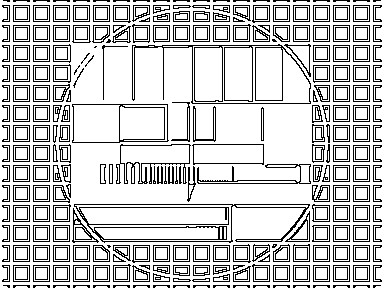
\includegraphics{l_o_g}}
     \end{minipage}
     \caption{Laplacian of Gaussian filter. Negative values
       are black and positive values are white\label{fig:log}}
   \end{center} % Generiere Balken mit Beschriftung mithilfe von RMagick?
\end{figure}
The property of the Laplacian of Gaussian is that it has zero-crossings
at edge locations. These zero-crossings can be detected by using morphological
operations as shown in \cite{RefWorks:356} or by using a combination of
thresholding, dilation, and erosion.
While edge detection using Laplacian of Gaussian is not straightforward
to implement, it has the interesting property that it always yields closed
contours since the edges are defined as an iso-line of a two-dimensional
function.

The detection of zero-crossings was not implemented at the time of writing
this report. The implementation of the LoG filter using \emph{HornetsEye} is
as follows
\begin{scriptsize}
  \verbatiminput{l_o_g.rb}
\end{scriptsize}

% \section{Registration/tracking}
% Moreover, it is important to understand that tracking error is not analogous
% to the Rayleigh criterion, i.e. it is not a constant measured in nanometers
% for the particular microscope con?guration. Instead it depends strongly on
% the signal intensity, that is, the contrast between the particle and its
% surroundings.
% Shape based recognition: 27
% Coarse-to-fine localisation (285)
% (particle filtering (427))
% $\ldots$

% \subsection{Geometric hashing}
% \cite{RefWorks:59} (39,40,38,312)
% $\ldots$

% \subsection{Random Sample Consensus}
% \cite{RefWorks:92} (84,31,315)
% $\ldots$

% \subsection{Locality Sensitive Hashing}
% \cite{RefWorks:317}, (316,83,33) databases by Mayur Indyk
% Scale- and rotational invariant shape context \cite{RefWorks:26}
% $\ldots$

% \subsection{Bounded Hough Transform}
% Wedekind \cite{Refworks:431}, (Wiener Filter?)
% \cite{RefWorks:36}
% Adaptive size of grid for different speed/resolution
% Estimating 3-D rigid body transform \cite{RefWorks:292}
% $\ldots$

\section{Implementation}
Most larger software packages offer a scripting interface. Sometimes bindings
for a specific scripting language are provided. In other cases the
functionality of the software is available as interfaces within a
component-oriented system such as DCOM, CORBA, SOAP, or other. Here the
approach of implementing bindings for the scripting language called
Ruby\footnote{\url{http://www.ruby-lang.org/}} was chosen
because it is a pure object-oriented, dynamically typed language. The
reference implementation is free and open source and it runs under GNU/Linux,
Microsoft Windows, and other platforms. Furthermore bindings for many
libraries are available already. The language is dynamically typed which makes
it easier to use and integrate existing bindings with conflicting datatypes.
Dynamic languages with meta-programming facilities such as Smalltalk,
LISP, Python, and Ruby are known for their capability to cope with
complexity.\cite{RefWorks:311}. Ruby features code blocks which is a
unifying concept for loops, function objects, and iterators.

Figure
\ref{fig:architecture} shows the current state of the
architecture which is being developed in context of this work.% report early
\begin{figure}[htbp]
   \begin{center}
     \resizebox{.7\textwidth}{!}{\includegraphics{architecture}}\\
     \caption{Software architecture of machine vision system\label{fig:architecture}}
   \end{center}
\end{figure}
A Ruby-extension \emph{HornetsEye} is being implemented which integrates
the functionality of several GPL-software packages and makes use of it. As one
can see in figure \ref{fig:architecture}, wherever possible
existing GPL software packages were integrated instead of implementing a custom
solution.
\begin{itemize}
\item {\bf Boost}: The Boost Library\footnote{\url{http://www.boost.org/}}
  offers smart pointers to do exception safe programming, multi-dimensional
  arrays, template meta-programming, abstract data types for linear algebra
  and many other programming concepts. The Boost library is going to be part
  of a future C++ standard.
\item {\bf OpenGL}: OpenGL can be used to display images and videos.
\item {\bf V4L}: Video for Linux provides access to many video sources
  such as USB-cameras and frame grabbers.
\item {\bf libdc1394}: libdc1394\footnote{\url{http://damien.douxchamps.net/ieee1394/libdc1394/}}
  is used to access IIDC/DCAM-compliant firewire digital cameras.
\item {\bf XVideo}: XVideo is used to display images and videos using
  2-D hardware acceleration. This is the fastest way of displaying images
  on a PC.
\item {\bf Xine}: Using Xine\footnote{\url{http://www.xinehq.de/}} one can
  read virtually any video file and it is even possible to read streaming
  videos.
\item {\bf OpenEXR}: The OpenEXR library\footnote{\url{http://www.openexr.org/}}
  is used for saving and loading high dynamic range images.
\item {\bf fftw3}: The fftw3\footnote{\url{http://www.fftw.org/}}-library
  is maybe the fastest library for performing discrete Fourier transforms. It
  can be invoked by using Masahiro Tanaka's Ruby-extension
  NArray-fftw3\footnote{\url{http://narray.rubyforge.org/}}.
\item {\bf RMagick}: The RMagick\footnote{\url{http://rmagick.rubyforge.org/}}
  Ruby-extension allows one to use the powerful ImageMagick/Magick++\footnote{\url{http://www.imagemagick.org/Magick++/}}
  library in Ruby for loading and saving images.
\end{itemize}
There are further libraries which are useful to develop a complete application
including a graphical user interface
\begin{itemize}
\item {\bf Qt4Ruby}: Qt4Ruby\footnote{\url{http://rubyforge.org/projects/korundum/}}
  can be used to develop graphical user interfaces.
\item {\bf rgplot}: rgplot allows one to use gnuplot\footnote{\url{http://www.gnuplot.info/}} from within Ruby to plot functions.
\item {\bf Natural Docs}: Natural Docs\footnote{\url{http://www.naturaldocs.org/}}
  is used to create the HTML documentation.
\item {\bf RDoc}: RDoc\footnote{\url{http://www.ruby-doc.org/stdlib/libdoc/rdoc/rdoc/}}
  is used to create documentation for the interactive Ruby shell.
\item {\bf IRB/FXRI}: IRB and FXRI are interactive Ruby shells.
\end{itemize}
Some of these software packages do not run under Microsoft Windows. Therefore
alternate libraries need to be integrated for being able to run the
higher level code on both platforms. Currently it is planned to
use Direct3D, DirectShow, CMU1394, DXVA, and Microsoft Mediaplayer as alternate
libraries on the Microsoft Windows platform. Porting has only
begun at the time of writing this report. Figure \ref{fig:platforms} shows an
early result of these efforts.
\begin{figure}[htbp]
   \begin{center}
     \begin{minipage}[c]{.45\textwidth}
       \resizebox{\textwidth}{!}{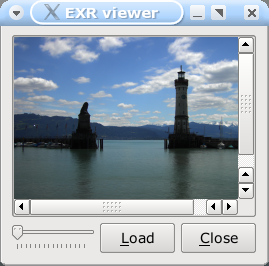
\includegraphics{linux}}
     \end{minipage}
     \begin{minipage}[c]{.45\textwidth}
       \resizebox{\textwidth}{!}{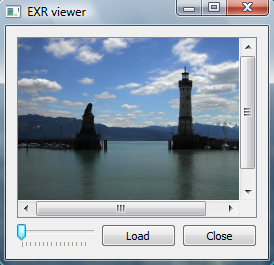
\includegraphics{windows}}
     \end{minipage}
     \caption{Ruby application running under GNU/Linux as well as Microsoft Windows\label{fig:platforms}}
   \end{center}
\end{figure}

% low-level, high-level
% multi-arrays, mpl

% \cite{RefWorks:296} Qt designer
% \cite{RefWorks:378}
% Denker's paper (311), Ruby: Perl like syntax, many libraries (no own ide)

% ruby optimizer not available (YARV,strongtalk), knowledge all elements in an
% array of same type

\chapter{Conclusion}
Most optical microscopes and TEMs offer a serial interface for control.
Also some digital cameras are accessible by means of a standardised interface
such as IIDC/DCAM (standard supported by many firewire cameras) or other.
A powerful platform for research work becomes feasible where public
documentation for hardware is available. It is in the interest of the
individual researcher to ascertain these requirements when purchasing
equipment.

It was pointed out in the introduction  that the microfactory of the
future will likely require machine vision for feedback control.
Hollis\cite{RefWorks:154},\cite{RefWorks:155} shows development of a
micro-factory doing vision-guided precision assembly.
Brequet\cite{RefWorks:262} gives an overview of rapid prototyping techniques.
Whether the desktop factory will become reality remains to be seen, but a
system capable of automated manufacturement and assembly of components of
a single material could be the next step towards this goal.

The expected original contributions from this research includes
\begin{itemize}
\item novel methods for feature-extraction and/or object-recognition in
  microscopy images (low depth of field)
\item an original approach for manipulating videos and images
\item an implementation of a machine vision system with an unprecedented
  degree of hardware integration
\end{itemize}

% TEM
% optical microscope
% research ignoring political, economical, and social developments.
%   -> contribution to solve this problem
% THANKS!!!
% Currently the MMVL is engaged in the EPSRC Nanorobotics project
% (grant no. GR/S85689/01). The task of the MMVL is to develop an automated
% vision feedback system to control the position and function of a
% nanomanipulator inside a TEM environment (see figure \ref{fig:jeol})
% using real-time analysis of
% electron/ion images. The work package further includes the development and
% integration of new vision methods with a microscope mounted digital camera
% system, that provides feedback to the nanomanipulation and nanopositioning
% control electronics.
% Optimisation of dynamic language will make a lot of this work redundant

\appendix
\chapter{Appendix}
\section{Spectral factorisation with Laguerre}\label{cha:laguerre}
Laguerre's algorithm (see algorithm \ref{alg:laguerre}) is a numerical
method for determining the roots of a polynomial $p:\mathbb{C}\to\mathbb{C}$. 
\begin{algorithm}[tbhp]
  \caption{Laguerre's method for finding a single root of
    a polynomial\cite{Refworks:406}\label{alg:laguerre}}
  \KwIn{Polynomial $p(x)$}
  \KwOut{A zero crossing $o\in\mathbb{C}$ of $p$}
  \tcc{Initialise $x\in\mathbb{C}$ with an arbitrary value. $c$ is a counter
  to ensure termination}
  $x\mapsto 0.0+0.0\,i$; $c\mapsto 100$\;
  \While{$c\ge 0$}{
    \If{$\left|p(x)\right|$ sufficiently small}{
      \Return{$x$}\;
    }
    $g=p^\prime(x)/p(x)$; $h=g^2-p^{\prime\prime}(x)/p(x)$\;
    \eIf{$\left|g+d\right|>\left|g-d\right|$}{
      $a=n/(g+d)$\;
    }{
      $a=n/(g-d)$\;
    }
    $x\mapsto x-a$; $c\mapsto c-1$\;
  }
\end{algorithm}
In practice computation of $g$ is always attempted instead of checking the
size of $\left|p(x)\right|$ first. If computation of $g$ fails
numerically, $\left|p(x)\right|$ is considered to be sufficiently small.
The number of iterations has to be restricted (\emph{e.g.} $100$) because
$x\mapsto x-a$ does not affect the numerical value of $x$ if $x\gg a$.
Laguerre's method usually converges on a root of the input polynomial
$p(x)$. To increase the reliability of the method one can add a fractional
step every so often to break possible limit cycles\cite{Refworks:406}.


\bibliographystyle{alpha}\bibliography{thesis}

\end{document}
\bye

% (structured light: 248, graycode http://www.abw-3d.de  http://apollo.fh-nuertingen.de/%7Eag3d/lit/wolf2_97.zip)
% (boosting \cite{RefWorks:305})
% (computer algebra (369,376)) !!!
% (3-D descriptors (430))
% (combining SFM SEM (260))
% (Nano-indentation (279))

% \chapter{State of the art}
%COMPOST?
% Pre- and postcondition, covariance, contravariance (G. Goos/W. Loewe)

% \subsection{Companies}
% \chapter{Suggested application areas}
% \subsection{Companies in microscopy}
% http://www.imas.co.uk/
% http://www.struers.com/
% http://www.alicona.com/
% http://www.bitplane.ch/
% http://www.ffa.co.uk/
% http://www.svi.nl/
% http://www.festo.com/ ?
% -> mimas/doc/otherprojects.dxx
% \begin{itemize}
% \item {\bf Kleindiek}\footnote{\url{http://www.nanotechnik.com/}}
% \item {\bf Diagnostic Products
%     Corporation}\footnote{\url{http://www.dpcweb.com/products/products.html}}:
%   Automation of laboratory tests, dilution, automatic reflex testing,
%   primary tube sampling, remote tests, allergy test, sample carousel,
%   ETA information, monitoring of reagents, supplies and waste
%   (expiration dates), washing, clot detection, refrigeration
% \item {\bf Sepro Robotique}\footnote{http://www.sepro-robotique.com/}:
%   Pick and place manipulators, robots
% \item {\bf RTS group}\url{http://www.rts-group.com/}
%   \emph{Lifescience}: Disposable tips, compound transfer, dispensing,
%     centrifugation, plate sealing/desealing, avoiding freeze/thaw cycles,
%     picking multiple valves, retrieval of cold samples ($-80^\circ C$),
%     samples stores/libraries, blood fractionation (red blood cells, white
%     cells, plasma), system \emph{integration}, sealing/cutting of tubes,
%     barcodes, database
% \item {\bf Fanuc Robotics}\footnote{\url{http://www.fanucrobotics.co.uk/}}:
%   standard industrial robotics, background editing, laser cutting, collision
%   detection, dynamics, tracking (robot operates on moving assembly line),
%   palletizing
% \item {\bf igm Robotic Systems, Inc.}\footnote{\url{http://www.igmusa.com/}}:
%   welding, cutting, beveling
% \item {\bf Allen Vanguard}\footnote{\url{http://www.allen-vanguard.com/}}:
%   BombTec Defender ROV, Vanguard Mk2 ROV,
%   bomp disposal, security equipment, endoscope, portable video microscopes
% \item Pacific Scientific\footnote{\url{http://www.pacsci.com/}}: High
%   performance motors for the Segway
% \item {\bf Bilsing Automation}\footnote{\url{http://www.bilsing-automation.com/}}
% \item {\bf M+T Welding Systems Ltd}\footnote{\url{http://www.m-and-t-welding.co.uk/}}:
%   electric/pneumatic tool changer, welding robots
% \item {\bf Cloos Schweisstechnik}\footnote{\url{http://www.cloos.de}}:
%   active/passive gas welding
% \item {\bf Kuka}\footnote{\url{http://www.kuka.de/}}: roboter-systeme,
%   offline programming, synchronisation for integration into a system, realtime
%   VxWorks, simulation/planning, visualisation, distributed components,
%   cable guides, linear translation platforms
% \item {\bf ASM Dimatec}\footnote{\url{http://www.asmgrupo.de/}}:
%   conveyor belt, toothed belt, rolls, gluing, welding, assembly
% \item {\bf Topometrix}\footnote{url{http://electron.mit.edu/~gsteele/mirrors/elchem.kaist.ac.kr/jhkwak/TopometrixWeb/TopoHome.htm}}:
%   Doing SPM inside an SEM.
% \item {\bf Omicron}\footnote{\url{http://www.omicron.de/}}: Complex systems
%   for doing surface science (deposition, analysis).
% \item {\bf Vecoo}\footnote{\url{http://www.veeco.com/}}: Combined SPM
%   and confocal scanning microscope.
% \item {\bf Zyvex}\footnote{\url{http://www.zyvex.com/Research/}}: This company
%   is doing research in MEMS and assembly by high precision robots.
% % http://www.roboticsonline.com/public/articles/articlesdetails.cfm?id=2635
% % http://www.preciseautomation.com/
% % http://www.motoman.com/
% % http://www.artificialmuscle.com/

% % [http://www.physikinstrumente.de/ Physik Instrumente Gmbh] - nanopositioning technology and motion control systems
% % [http://www.goodfellow.com/ Goodfellow] - metals and materials for research and industry
% % [http://www.kleindiek.com/ Kleindiek Nanotechnik]
% % [http://www.zyvex.com/Products/CMPM_001a.htm Zyvex microgripper]

% \item {\bf Coventor}\footnote{\url{http://www.coventor.com/}}: Development of
%   MEMS CAD software.
% \end{itemize}
% \subsection{Companies in rapid prototyping}
% \subsection{Micromanipulators}
% Etched (1990!): \cite{RefWorks:164}
% Adhesion: \cite{RefWorks:41}
% Freeze tweezers: \cite{RefWorks:249}
% Optical tweezers?
% dielectrophoresis 
% Breaking static friction: \cite{RefWorks:243}
% TEM manipulator \cite{RefWorks:255}
% Force sensing using strain gauges: \cite{RefWorks:187}


% \section{Cross-correlation}
% The position $\vec{p}:=\vec{OP}$ was estimated by using the following
% cross-correlation
% $\displaystyle\mathop{\operatorname{argmax}}_{\vec{\tau}\in\mathbb{R}}\int b_t\big(g(\vec{x})\big)\,b_t\big(t(\vec{x}-\vec{\tau})\big)\operatorname{d}\vec{x}$
% where $b_t(v)$ is defined as follows
% $b_t(v):=\left\{\begin{array}{ll}0 & v >= t\\1 & v < t\end{array}\right.$
% \begin{figure}[htbp]
%    \begin{center}
%      \resizebox{.8\textwidth}{!}{\includegraphics{tungstenCorrelation}}\\
%      \caption{Locating a tungsten tip by means of cross-correlation}
%    \end{center}
% \end{figure}
% \subsection{Linear Scale Invariant Filters}
% % Correlation <-> Convolution
% \subsubsection{Quantised Gauss filter}
% Accurate Gauss filters are computed by computing the integral of each
% sampling interval instead of taking samples of the Gauss function directly.
% The integral of the one-dimensional Gauss function is
% $\displaystyle\int\frac{1}{\sqrt{2\,\pi}|\sigma|}\,\e^{-\cfrac{x^2}{2\,\sigma^2}}\mathrm{d}x=\cfrac{1}{2}\,\mathrm{erf}\big(\cfrac{x}{\sqrt{2}\,|\sigma|}\big)$.
% In a similar manner accurate Gauss gradient filters are computed.
% \subsubsection{Laplacian of Gaussian}
% The Laplacian of Gaussian is defined as\\
% $L(x,y):=\nabla\big(G(x)\,G(y)\big)=\cfrac{\delta^2 G(x)}{\delta x^2}\,G(y)+
% G(x)\,\cfrac{\delta^2 G(y)}{\delta y^2}$
% with $G(x):=\int\frac{1}{\sqrt{2\,\pi}|\sigma|}\,\e^{-\cfrac{x^2}{2\,\sigma^2}}$.

% The accurate digital filter is defined using the integral\\
% $\displaystyle\int\int L(x,y)\mathrm{d}x\mathrm{d}y=\cfrac{\delta G(x)}{\delta x}\mathrm{erf}(y)+\cfrac{\delta G(y)}{\delta y}\mathrm{erf}(x)$.
% % See http://en.wikipedia.org/wiki/Scale_space
% % See http://en.wikipedia.org/wiki/Heat_equation
% \subsection{Canny}
% \subsection{Geometric hashing}
% \subsection{SIFT}
% \begin{figure}[htbp]
%   \begin{center}
%     \resizebox{.8\textwidth}{!}{\includegraphics{indentationSIFT}}\\
%     \caption{TEM image of indentation experiment with overlayed SIFT keys}
%   \end{center}
% \end{figure}
% SIFT keys, that agree on a potential model pose are identified using a
% Hough table\cite{RefWorks:85}. Key locations are maxima and minima of a
% difference of gaussian in a pyramid ($\Rightarrow$ only affected by
% distortion and noise). See algorithm \ref{alg:SIFT}.
% \begin{algorithm}
%   \KwIn{Input image}
%   \KwIn{Set of SIFT keys}
%   Expand input image by a factor of $2$ using bilinear interpolation\;
%   Apply a gauss-kernel with $\sigma=\sqrt{2}$\;
%   \While{image is big enough}{
%     Apply the gauss-kernel with $\sigma=\sqrt{2}$ again\;
%     Take the difference of these two images and add it to the pyramid\;
%     Subsample the last image with a pixel spacing of $1.5$ (requires a linear
%     combination of 4 adjacent pixels)\;
%   }
%   \ForEach{pixel in the pyramid}{
%     \eIf{pixel greater than its eight neighbours on the same pyramid level}{
%       \If{pixel is higher than the corresponding pixel off the next level}{
%         repeat computation on next level
%       }
%     }{
%       \If{pixel is lower than its eight neighbours on the same pyramid level}{
%         \If{pixel is lower than the corresponding pixel off the next level}{
%           repeat computation on next level
%         }
%       }
%     }}
%   Compute magnitude and orientation of Sobel gradient of each level of the
%   pyramid at each key location\;
%   Threshold gradient magnitudes at $0.1$ times the the maximum possible
%   gradient value\;
%   For each remaining key create a \unit[36]{bins} histogram of the local
%   gradient orientation of the image smoothed with 3 times the $\sigma$ of
%   the current pyramid level\;
%   After the histogram is smoothed, the peak of the histogram determines the
%   orientation of the SIFT key\;
%   \caption{Algorithm for locating SIFT keys\label{alg:SIFT}}
% \end{algorithm}
% \begin{figure}[htbp]
%   \begin{center}
%     \resizebox{.8\textwidth}{!}{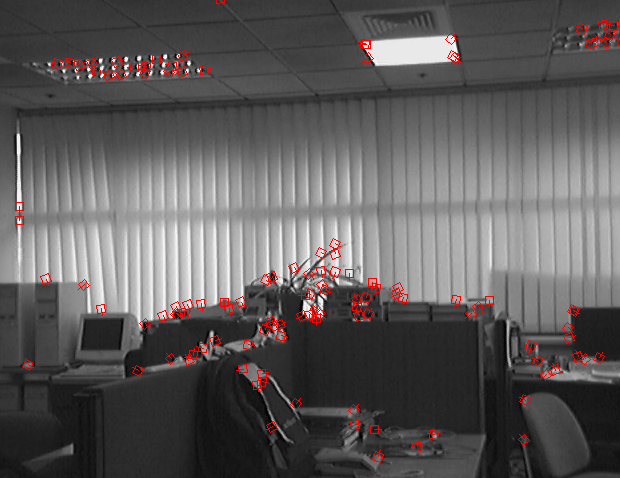
\includegraphics{sift1}}\\\medskip
%     \resizebox{.8\textwidth}{!}{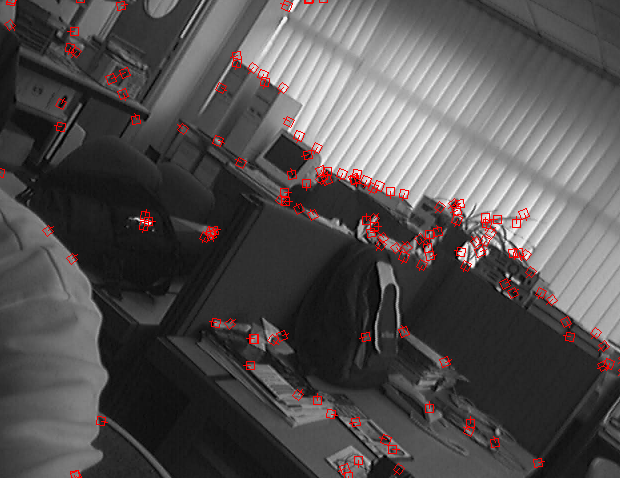
\includegraphics{sift2}}\\
%     \caption{SIFT extraction on two images to test rotational invariance}
%   \end{center}
% \end{figure}
% \subsection{Harris-Laplace detector}
% Keypoint localisation using the \emph{Harris-Laplace detector}
% detects Harris interestpoints at several scales and
% then selects the right scale by determining the maximum of the Laplacian
% function\cite{RefWorks:285}. In \cite{RefWorks:285} the Harris-Laplace detector
% is used to determine keypoints. Then the SIFT-descriptor is used to define a
% similarity measure between the features.
% \subsection{RANSAC}
% \subsection{Structure Tensors}
% \cite{RefWorks:280} gives a mathematical definition for structure tensors.
% \begin{defn}
%   A structure tensor $T\in\mathbb{R}^n\to K$ ($K$ being a suitable
%   representation space) is a continuous function fullfilling the following
%   conditions
%   \begin{itemize}
%   \item uniqueness constraint: $\forall\vec{x}\in\mathbb{R}^n: T(\vec{x})\overset{!}{=}T(-\vec{x})$
%   \item polar separability: $\exists f\in(\mathbb{R}\to\mathbb{R}):\forall\vec{x}\in\mathbb{R}^n:\|T(\vec{x})\|=f(\|\vec{x}\|)$
%   \item locally preserve angular metric: $\|\delta T\|=c\|\delta\vec{x}\|_{\|\vec{x}\|\mathrm{\ const.}}$
%   \end{itemize}
% \end{defn}
% For $n=2$ one can choose
% \begin{equation*}
%   T:=\left\{\begin{array}{rcl}\mathbb{R}^2 & \to & \mathbb{R}^{2\times 2}\\
%       \vec{x} & \mapsto & \vec{x}\,\vec{x}^\top\end{array}\right.
% \end{equation*}
% In contrast to defining a hyperplane (for $n=2$ a line) by
% $\vec{n}_1^\top\,\vec{x}=\vec{0},\|\vec{n}_1\|=1$, where there are two
% alternate definitions ($\vec{n}_2=-\vec{n}_1$), a structural
% tensor in 2-D allows one to find a mapping\cite{RefWorks:280}, which maps all
% vectors $\vec{x}\neq\vec{0}$ on the same tensor
% $T(\cfrac{\vec{x}}{\|\vec{x}\|})$.
% \subsection{Steerable filters}
% Let $f(\vec{x})$ be a 2-D filter ($\vec{x}\in\mathbb{R}^2$) and define
% $f^\theta$ as a rotated version of it
% \begin{equation*}
% f^\theta(\vec{x}):=f(\begin{pmatrix}\cos(\theta)&-\sin(\theta)\\
% \sin(\theta)&\cos(\theta)\end{pmatrix}\vec{x})
% \end{equation*}
% Then $f$ is steerable if (for any value of $\theta$) $f^\theta$ is a linear
% combination of a finite set of rotated versions of $f$
% \begin{equation*}
% f^\theta(\vec{x})=\displaystyle\sum_{j=1}^M k_j(\theta)\,f^{\theta_j}(\vec{x})
% \end{equation*}
% Most filters with a limited response are steerable according to
% \cite{RefWorks:276}. Therefore the response of a rotated filter can be computed
% analytic and exact using a filter-bench, which is superior to an \emph{ad-hoc}
% method of combining oriented filters.
% \subsection{Wavelets}
% \cite{RefWorks:270} and \cite{RefWorks:273} introduces the Quaternion-Wavelet
% transform. \cite{RefWorks:266} shows how to use Quaternion-Wavelets for
% disparity estimation. In \cite{RefWorks:294} quaternionic moments are used to
% recognise objects.


% \subsection{Other}
% \subsubsection{Angular Reconstitution}
% See \cite{RefWorks:256} and \cite{RefWorks:257} for details on reconstruction
% of molecules from multiple
% molecules\footnote{Also see \url{http://www.ecmjournal.org/}}.
% \subsubsection{Segmentation}
% Analysis of multivariate images and scatterplots can be applied
% to SEM images to visualise data (see \cite{RefWorks:258}). For example SEM
% and SPM images can be combined this way (see \cite{RefWorks:260}).

% Segmentation of lattice structures \cite{RefWorks:259}.

% \section{Micromanipulation}
% \subsection{Manipulators}
% Placing small solder-balls and components by fracture of the contact
% interface\cite{RefWorks:243}:
% \begin{itemize}
% \item Given:
%   \begin{itemize}
%   \item Glass needle coated with Au.
%   \item Glass plate coated with Au as substrate.
%   \item Silica spheres
%   \item Multi-axial force-controlled sensor
%   \end{itemize}
% \item Result:
%   \begin{itemize}
%   \item Second order forces are dominant (adhesion by Van-der-Vaals,
%     electrostatic and capillary forces). \cite{RefWorks:41} offers
%     some formulas for estimating adhesive forces.
%   \item Irreversible increase of adhesional force caused by electron beam
%     makes it very difficult to achieve repeatability.
%   \item Pick and place possible by fracture of the contact interface.
%   \end{itemize}
% \end{itemize}

% In \cite{RefWorks:249} freeze tweezers are presented. The object is picked
% up by creating a thin layer of ice. Cooling is achieved by expansion of Helium.

% According to \cite{RefWorks:250} microactuators can be categorised into
% \begin{itemize}
% % are inchworm, stick-slip both inertial drives? (->RefWorks:262)
% \item inchworm motors
% \item stick-slip actuators or impact actuators
%   (using an impulse to overcome static friction)
%   \begin{itemize}
%   \item electromagnetical
%   \item piezoelectrical
%   \item phototermal
%   \item electrostatic
%   \end{itemize}
% \item monolitic actuators (see \cite{RefWorks:262})
% \end{itemize}

% Force-feedback is desirable. According to \cite{RefWorks:253} even nano-scale
% objects can be manipulated with grippers (carbon nanotube tweezers).
% \cite{RefWorks:253} explains how to microfabricate electro-thermally actuated
% force-feedback grippers\footnote{Also see \url{http://www.mic.dtu.dk/},
%   \url{http://www2.mic.dtu.dk/} and \url{http://www.danchip.dtu.dk/}}.

% \cite{RefWorks:255} describes a nano-manipulator developed at
% Fukuda Lab\footnote{See \url{http://www.mein.nagoya-u.ac.jp/}}, which can be
% used in a TEM as well as an SEM.

% \subsection{Micro-factories}
% \cite{RefWorks:262} gives an explanation of the two approaches:
% \begin{itemize}
% \item The {\bf bottom-up} approach means building up components
%   molecule by molecule.
% \item The {\bf top-down} approach denotifies machining components from raw
%   material and assembling them. This rather ``conventional'' approach ideally
%   would make use of the industries' concept of rapid-prototyping (RP), so that
%   all required parts can be produced within the micro-factory.
% \end{itemize}
% While it is unsure, wether the {\bf bottom-up} approach feasible at all,
% \cite{RefWorks:262} gives some tangible ideas, how future {\bf top-down}
% systems will look like.
% \begin{itemize}
% \item Micro \emph{electro discharge machining} (EDM)
% \item Micro \emph{stereo-litography}\footnote{\url{http://www.cmf.rl.ac.uk/latest/msl.html}} using light-induced polymerisation. A resolution of
%   \unit[5]{$\mu\mathrm{m}$} was reached!
%   % STL: stereo litography file format.
% \item \emph{Selective laser sintering} (polymers, metals or ceramics) has a
%   lower resolution of \unit[100]{$\mu\mathrm{m}$} at the moment.
% \item \emph{three dimensional printing} (3DP) can be used to dispense
%   solder or adhesives.
% \item \emph{Laser forming} can be used to bend objects or sculpt
%   surfaces\footnote{\url{http://www.twi.co.uk/j32k/unprotected/band_1/surfi-sculpt_index.html}}
% \end{itemize}

% \appendix
% \chapter{Appendix}
% \section{MinGW}
% \subsection{Simple example}
% \url{http://mirzam.it.vu.nl/mingw/}\\
% \url{http://dev.panopticsearch.com/cross-compile.html}\\
% \url{http://www.mingw.org/}\\
% \url{http://silmor.de/29}\\
% \url{http://sourceforge.net/projects/qtwin/}\\
% \url{http://www.technosis.de/mingw/crosscompile/}\\
% \url{http://lists.trolltech.com/qt-interest/2006-01/msg00289.html}\\
% \url{http://doc.trolltech.com/4.1/qmake-reference.html}\\
% \url{http://gentoo-wiki.com/HOWTO\_Install\_GoogleEarth\_with\_wine}\\
% \url{http://corefonts.sourceforge.net/}

% Under Linux:
% build-cross.sh (more than 512 MByte disk-space).\\
% The installation will be about 155 MByte.\\
% \\
% Under Windows:\\
% 1. Download and install\\
% http://prdownloads.sf.net/mingw/MinGW-4.1.0.exe?download\\
% \\
% 2. Download and unzip this file from trolltech:\\
%     qt-win-opensource-src-4.1.1.zip\\
% \\
% 3. Copy all the files and folder under directory\\
% "qt-win-opensource-src-4.1.1" to a folder where you like to perform\\
% installation.\\
% In my case it was C:$\backslash$Qt$\backslash$4.1.1$\backslash$\\
% \\
% 4. Open command line and cd to that folder e.g. "cd C:$\backslash$Qt$\backslash$4.1.1$\backslash$"\\
% Add path to MinGW (e.g. SET PATH=\%PATH\%;C:$\backslash$MinGW$\backslash$bin)\\
% \\
% 5. Next type in "configure -platform win32-g++"\\
% If you need to configure further, then give the command "configure -help"\\
% and turn on/off appropriate options, else above should just work fine in\\
% pretty much all cases.\\
% \\
% 5. Hit "y/Y" to accept the License agreement.\\
% \\
% 6. Once Configure script ends, type in "mingw32-make"\\
% This process took 3.5 hours on my 1.4 GHz Xeon machine so expect that much\\
% time.\\
% \\
% 7. One last step is to set the PATH environment variable to include\\
% "c:$\backslash$Qt$\backslash$4.1.1$\backslash$bin".\\
% \\
% That's it folks!!!!\\
% \\
% Special thanks to Huber, George for the pointer "-platform win32-g++".\\
% Thanks.\\
% Paresh Patel\\
% \\
% Clean up things: Search and delete the following files:*.o\\
% Search and delete the following directories: tmp,debug*\\
% This will leave a bit more than 1 GByte\\
% \\
% Under Linux:\\
% Copy the C:$\backslash$Qt$\backslash$4.1.1$\backslash$ directory to /opt/cross/Qt/4.1.1\\
% Delete the following files and directories: doc,lib/*d4.a,lib*d.a,lib/*.dll,\\
% bin/*d4.dll\\
% \\
% This will leave you 180 MByte of Qt-files.\\
% \\
% Put links:\\
% cd /opt/cross/i386-mingw32msvc/include\\
% ln -s ../../Qt/4.1.1/include/* .\\
% cd /opt/cross/i386-mingw32msvc/lib\\
% ln -s ../../Qt/4.1.1/lib/*.a .\\
% \\
% Link Qt- and mingw-DLL's into current directory.\\
% Create desired Qt*.pc files for cross-compiler tree\\
% \\
% Create installer with "wine nsis.exe"\\
% \\
% Create CD:\\
% mkisofs -o /tmp/cross.iso -f -joliet-long mingw\\

% Autorun.inf:\\
% \begin{verbatim}
% [autorun]
% open = HelloInstaller.exe
% \end{verbatim}

% \subsection{Mimas}
% \begin{itemize}
% \item Install boost
% \item Cross-compile popt, fftw
% \item Cross-compile minimal ImageMagick++
% \begin{itemize}
% \item Add have\_magick\_plus\_plus='yes' to configure.ac to force build of Magick++.
% \item Run autoconf
% \item LD\_LIBRARY\_PATH=/opt/cross/i386-mingw32msvc/lib PATH=\$PATH:/opt/cross/i386-mingw32msvc/bin ./configure --enable-delegate-build --disable-shared --without-perl --disable-largefile --with-x=no --with-magick-plus-plus=yes --host=i386-mingw32msvc --prefix=/opt/cross/i386-mingw32msvc
% \item Re-enable defines in magick/magick-config.h
% \begin{itemize}
% \item HAVE\_MALLOC
% \item HAVE\_REALLOC
% \end{itemize}
% \item Remove macros changing malloc and realloc in magick/magick-config.h
% \item Remove call to AnimateImages(wand->image\_info,wand->images) in wand/magick-image.c
% \end{itemize}
% \end{itemize}

% Choose appropriate images in final thesis (microscope images?)

% How to use algorithm style for Ruby code?

% \section{Quaternions}
% Quaternions are numbers of the form
% $q=q_0+iq_1jq_2kq_3$ where $q_l\in\mathbb{R}$,
% $l\in\left\{0,1,2,3\right\}$ and $i$, $j$, $k$
% are obeying the multiplicative rules
% $ij=ji=-k$ and
% $i^2=j^2=k^2=-1$\cite{RefWorks:270}.
% $(\mathbb{H},+,*)$ is a non-commutative ring.
% \begin{figure}[htb]
%   \begin{center}
%     \begin{tabular}{|r||r|r|r|r|}\hline
%           &  $1$ &  $i$ &  $j$ &  $k$ \\\hline\hline
%       $1$ &  $1$ &  $i$ &  $j$ &  $k$ \\\hline
%       $i$ &  $i$ & $-1$ &  $k$ & $-j$ \\\hline
%       $j$ &  $j$ & $-k$ & $-1$ &  $i$ \\\hline
%       $k$ &  $k$ &  $j$ & $-i$ & $-1$ \\\hline
%     \end{tabular}
%     \caption{Multiplication table for Quaternions\cite{RefWorks:270}}
%   \end{center}
% \end{figure}

% The product of two pure quaternions\footnote{$q\in\mathbb{H}$ is pure
%   $:\Leftrightarrow$ real part of $q$ is zero} combines in itself the
% scalar-product as well as the vector cross-product\cite{RefWorks:270}:
% \begin{align*}
%   qr=&(-q_1r_1-q_2r_2-q_3r_3)\\
%      &+i(q_2r_3-q_3r_2)\\
%      &+j(q_3r_1-q_1r_3)\\
%      &+k(q_1r_2-q_2r_1)
% \end{align*}
% A unit quaternion $q\in S^3:=\left\{q\in\mathbb{H}|\left|q\right|=1\right\}$
% can be seen as a rotation of $2\theta$ around the axis
% $\begin{pmatrix}q_1\\q_2\\q_3\end{pmatrix}$, where
% $q=\cos(\theta)+\sin(\theta)n$ with $n\in\mathbb{H}$ pure. Note, that
% $q$ and $-q$ are representing the same rotation.
% % Rodriguez Matrix and Euler representation: corresponding rotation matrix ->
% % Mathematical handbook!

% \section{Hartley transform}
% The Hartley transform of a function $f(t)$ is defined by
% \footnote{\url{http://en.wikipedia.org/wiki/Hartley_transform}}:
% \begin{equation*}
% \mathcal{H}\left\{f\right\}(\omega):=\cfrac{1}{\sqrt{2\pi}}\int_{-\infty}^\infty
% f(t) \operatorname{cas}(\omega t) \operatorname{d}t
% \end{equation*}
% where
% \begin{equation*}
% \operatorname{cas}(t):=\cos(t) + \sin(t) = \sqrt{2} \sin (t+\pi /4)
% \end{equation*}
% The Hartley transform is its own inverse
% \begin{equation*}
% f=\mathcal{H}\left\{\mathcal{H}\left\{f\right\}\right\}
% \end{equation*}
% \section{Fourier transform}
% % Fourier transform <-> Eigen transform
% The (non-unitary) 1-D fourier-transform is defined as
% follows\footnote{\url{http://en.wikipedia.org/wiki/Continuous_Fourier_transform}}
% \begin{align*}
%   f&\fourier F\\
% \displaystyle F(\omega)&:=\int_{-\infty}^\infty f(t)\,\e^{-i\omega t}\,\operatorname{d}t\\
% \displaystyle f(t)&:=\cfrac{1}{2\pi}\int_{-\infty}^\infty F(\omega)\,\e^{i\omega t}\,\operatorname{d}\omega
% \end{align*}
% with $i^2=-1$.
% \section{Z-transform}
% The (bilateral) Z-transform of a discrete time signal $(x)$ is\footnote{\url{http://en.wikipedia.org/wiki/Z-transform}}
% \begin{equation*}
%   Z\{(x)\}(z)=\displaystyle{\sum}_{i=0}^\infty x_i\,z^{-i}
% \end{equation*}
% The inverse Z-transform is defined by
% \begin{equation*}
%   Z^{-1}\{(X)\}(i)=\frac{1}{2 \pi j} \oint_{C} X(z) z^{i-1} dz 
% \end{equation*}
% where $C$ is a counterclockwise closed path encircling the origin and entirely
% in the region of convergence.
% If $C$ is the unit circle, the integral simplifies to
% \begin{equation*}
%   \frac{1}{2 \pi} \int_{-\pi}^{+\pi} X(e^{j \omega}) e^{j \omega i} d \omega
% \end{equation*}
% \section{Quaternion Fourier Transform}
% The 2-D quaternionic Fourier transform is defined as
% \begin{defn}
%   $f\overset{\mathbb{H}}{\fourier}F^q\\
%   F^q(\vec{u}):=\displaystyle\int_{\mathbb{R}^2}\e^{-i2\pi u_1x_1}f(\vec{x})\e^{-j2\pi u_2x_2}\operatorname{d}^2\vec{x}$ with $\vec{x},\vec{u}\in\mathbb{R}^2\\
%   f(\vec{x})=\displaystyle\int_{\mathbb{R}^2}\e^{i2\pi u_1x_1}F^q(\vec{u})\e^{j2\pi u_2x_2}\operatorname{d}^2\vec{u}$
% \end{defn}
% \section{Laplace's equation}
% \emph{Laplace's equation} is a partial differential equation named after its
% discoverer Pierre-Simon Laplace. The solutions of Laplace's equation are
% important in many fields of science, notably the fields of
% electromagnetism, astronomy, and fluid dynamics, because they describe the
% behavior of electric, gravitational, and fluid potentials.

% In three dimensions, the problem is to find twice-differentiable real-valued
% functions $\phi$ of real variables $x$, $y$ and $z$ such that
% \begin{equation*}
% {\frac{\partial^2 \varphi}{\partial x^2}} +
% {\frac{\partial^2 \varphi}{\partial y^2}} +
% {\frac{\partial^2 \varphi}{\partial z^2}} = 0.
% \end{equation*}

% This is often written as
% $\nabla^2 \varphi = 0$

% or

% $\operatorname{div}\,\operatorname{grad}\,\varphi = 0 $,

% where $\operatorname{div}$ is the divergence and $\operatorname{grad}$ is the
% gradient, or

% $\Delta \varphi = 0$

% where $\Delta$ is the Laplace operator.
% \footnote{\url{http://en.wikipedia.org/wiki/Laplace\%27s_equation}}
% \subsection{Harmonic function}
% A harmonic function is a twice continuous differentiable function,
% $f:U\to\mathbb{R}$ (where $U$ is an open subset of $\mathbb{R}^n$) which
% satisfies the Laplacian equation, \emph{i.e.}
% \footnote{\url{http://en.wikipedia.org/wiki/Harmonic_function}}
% \begin{equation*}
% \displaystyle\sum_{i=1}^{n}
% {\frac{\partial^2 \varphi}{\partial x_1^2}} +
% {\frac{\partial^2 \varphi}{\partial x_2^2}} +
% \ldots
% +
% {\partial^2 \varphi\over \partial x_n^2 } = 0
% \end{equation*}
% \subsection{Gabor filter}
% \begin{figure}[htb]
%   \begin{center}
%     \resizebox{.6\textwidth}{!}{\includegraphics{gabor}}\\
%     \caption{Real and complex part of 1D Gabor filter, $\sigma=2$, $k=3$}
%   \end{center}
% \end{figure}
% A Gabor filter is a linear shift-invariant filter, whose impulse response
% is defined by a harmonic function multiplied by a Gaussian function
% \footnote{\url{http://en.wikipedia.org/wiki/Gabor_filter}}
% \begin{equation*}
% g(x):=\cfrac{1}{\sqrt{2\pi}\left|\sigma\right|}\,
% \e^{-\cfrac{x^2}{2\sigma^2}}\,
% \e^{ikx}
% \end{equation*}
% with $i^2=-1$.
% % Gabor filters are not separable in frequency and orientation?
% % See \cite{Refworks:278}
% Gabor filters have been applied successfully to do texture
% segmentation\cite{RefWorks:284}.
% \begin{figure}[htb]
%   \begin{center}
%     \resizebox{.6\textwidth}{!}{\includegraphics{gaborF}}\\
%     \caption{Fourier transform of the 1D Gabor filter, $\sigma=2$, $k=3$}
%   \end{center}
% \end{figure}
% The fourier transform of the gabor filter is
% \begin{equation*}
%   G(\omega)=\left|\sigma\right|\e^{\cfrac{-\sigma^2(\omega-k)^2}{2}}
% \end{equation*}
% \subsection{Spherical Harmonics}
% \emph{Laplace's equation} also can be written in spherical coordinates\footnote{\url{http://en.wikipedia.org/wiki/Spherical_harmonics}}
% \begin{equation*}
% {1 \over r^2}{\partial \over \partial r}\left(r^2 {\partial f \over \partial r}\right)
%   + {1 \over r^2\sin\theta}{\partial \over \partial \theta}\left(\sin\theta {\partial f \over \partial \theta}\right) 
%   + {1 \over r^2\sin^2\theta}{\partial^2 f \over \partial \varphi^2} = 0
% \end{equation*}
% where
% \begin{equation*}
% \left[\begin{matrix}
%     x & = & r\sin\theta\cos\phi \\
%     y & = & r\sin\theta\sin\phi \\
%     z & = & r\cos\theta \end{matrix}\right.
% \end{equation*}

% \section{Hilbert transform}
% The \emph{Hilbert transform}, here denoted $\mathcal{H}$, of a real-valued
% function, $s(t)$, is obtained by convolving signal $s(t)$ with $1/(\pi t)$ to
% obtain $\widehat s(t)$:\footnote{\url{http://en.wikipedia.org/wiki/Hilbert_transform}}
% \begin{equation*}
% \widehat s(t) = \mathcal{H}\left\{s\right\}(t) = (h*s)(t) =
% \cfrac{1}{\pi}\int_{-\infty}^{\infty}\cfrac{s(\tau)}{t-\tau}\, d\tau
% \end{equation*}
% The discrete Hilbert transform
% \begin{equation*}
% h[n]=\begin{cases}
%   0, & \mbox{for }n\mbox{ even},\\
%   \cfrac2{\pi n} & \mbox{for }n\mbox{ odd}
% \end{cases}
% \end{equation*}
% has the following Fourier transform
% \begin{equation*}
% H(\e^{j\omega}) = 
% \begin{cases}
% +j, & -\pi \leq \omega < 0 \\
% -j, & 0 \leq \omega < \pi
% \end{cases}
% \end{equation*}

% % Hilbert transform of sin(x) is -cos(x). The transform can be used to
% % create a complex valued signal from a real signal.

% Thomson Gale: Collection of  eighteenth century books and the Times archive
% FAME: Company information
% Digimap Ordnance Survey: Digital maps of UK
% IMechE proceedings archive http://archive.pepublishing.com/
% Nasa vision group: http://vision.arc.nasa.gov/publications.html
% Kiel vision group: http://www.ks.informatik.uni-kiel.de/
% Knutssen: http://www.imt.liu.se/mi/Publications/phdtheses.html
% I-Swarm robots: http://www.swarmrobot.org/

% Books
% Nanosystems               620    DR (LEVEL 3)
% The Mechatronics Handbook 629.89 ME (LEVEL 3)
% Mathematical Handbook for 510    KO (LEVEL 2)
% scientists and engineers

% Signal Processing for Computer Vision, Knutssen, Granlund

% difference of Poisson filters bandpass, lognormal bandpass
% hierarchical state machines

% http://math.ucsd.edu/~jeggers/latex/amsthdoc.pdf
% http://www.tug.org/tex-archive/info/symbols/comprehensive/symbols-a4.pdf
% http://www.ctan.org/tex-archive/macros/latex/contrib/trfsigns/
% http://vision.ece.ucsb.edu/ Santa Barbara Computer Vision Lab

% Open source vision software lowering cost of research
% A new version of the Mimas software from Sheffield Hallam University has been released. It was conceived as a platform for real-time machine vision research, and its aim is to reduce the turnaround time of new research. Mimas has been used to build a number of vision systems, including for two European Union sponsored projects, namely MINIMAN and MiCRoN, and is currently being used in the EPSRC funded Nanorobotics contract. Mimas is also being used to build a number of customised vision solutions for academia and industry. The package is available for free download under the LGPL licence.
% Choose good datatypes for library

% http://en.wikipedia.org/wiki/Artificial_neural_network
% http://en.wikipedia.org/wiki/Markov_decision_process
% http://en.wikipedia.org/wiki/RANSAC, Refworks: 92, 84, 314, 315, 323

% Discrete FIR Wiener filter:
% http://en.wikipedia.org/wiki/Wiener_filter
% From The MIT Press Classics Series:
% Extrapolation, Interpolation, and Smoothing of Stationary Time Series
% Norbert Wiener
% Siehe Levinson-Durbin Algorithms zur Loesung von Toeplitz-Inverse


% http://www.mit.edu/~vona/LSH/LSH.html

% http://docs.python.org/ref/node33.html (old-style <-> new-style classes)

% Microassembly: http://www.sandia.gov/isrc/precmicroassy.html
% Gluing and UV-hardening: http://robotics.eecs.berkeley.edu/~ronf/milli-robot.html

% Huertas: (RefWorks:356) patterns
% 0+0
% +00
% 000

% Wiener-Khinchin: autocorrelation = Fourier-transform of absolute square of
% energy
% http://mathworld.wolfram.com/Wiener-KhinchinTheorem.html

% http://planetmath.org/ !!!

% Splitting circle method: http://en.wikipedia.org/wiki/Splitting_circle_method

% -------------------------------

% Camera Calibration:
% Let <math>\vec{m}_i\in\mathbb{R}^3,\,i\in\{1,2,\ldots,N\}</math> be the [http://en.wikipedia.org/wiki/Homogeneous_coordinates#Use_in_computer_graphics homogeneous coordinate] of the <math>i</math>th point on the planar calibration-object and let <math>\vec{m}^\prime_i\in\mathbb{R}^3</math> be the homogeneous coordinate of the corresponding pixel in the camera-image. Further let <math>(\mathbb{R}^n,\simeq)</math> be an [http://en.wikipedia.org/wiki/Equivalence_relation equivalence relation] defined by

% <math>
% \vec{a}\simeq\vec{b}\ :\Leftrightarrow\ \exists\lambda\in\mathbb{R}/\{0\}:\,\lambda\,\vec{a}=\vec{b}
% </math>

% If the camera-system does an ideal central projection (e.g. no distortion), the projective transformation (the [http://en.wikipedia.org/wiki/Homography Homography]) can be modelled using <math>\mathcal{H}\in\mathbb{R}^{3\times 3}</math> as follows

% <math>
% \vec{m^\prime}_i+\vec{\epsilon}_i\simeq\mathcal{H}\vec{m}_i
% </math>

% or more elaborately
% <math>
% \lambda\,\begin{pmatrix}m^\prime_{i1}\\m^\prime_{i2}\\m^\prime_{i3}\end{pmatrix}+
% \begin{pmatrix}\epsilon_{i1}\\\epsilon_{i2}\\\epsilon_{i3}\end{pmatrix}=
% \begin{pmatrix}h_{11}&h_{12}&h_{13}\\h_{21}&h_{22}&h_{23}\\h_{31}&h_{32}&h_{33}\end{pmatrix}\,
% \begin{pmatrix}m_{i1}\\m_{i2}\\m_{i3}\end{pmatrix}
% </math>
% where <math>(\epsilon_{i1},\epsilon_{i2})^\top</math> is the zero-mean error-vector in the observation of the <math>i</math>th point in the camera-image.

% Using <math>m_{i3}=m^\prime_{i3}=1,\ \epsilon_{i3}=0</math> and <math>\vec{h_i}^\top=\begin{pmatrix}h_{i1}&h_{i2}&h_{i3}\end{pmatrix},\ i\in\{1,2,3\}</math> the
% model can be reformulated to
% <math>
% \begin{pmatrix}m^\prime_{i1}\\m^\prime_{i2}\end{pmatrix}=\cfrac{1}{\vec{h_3}^\top\cdot\vec{m}_i}\,
% \begin{pmatrix}\vec{h_1}^\top\\\vec{h_2}^\top\end{pmatrix}\,
% \begin{pmatrix}m_{i1}\\m_{i2}\\1\end{pmatrix}-
% \begin{pmatrix}\epsilon_{i1}\\\epsilon_{i2}\end{pmatrix}
% </math> or <math>
% \begin{pmatrix}m^\prime_{i1}\\m^\prime_{i2}\end{pmatrix}\,\big(\vec{h_3}^\top\cdot\vec{m}_i\big)=
% \begin{pmatrix}\vec{h_1}^\top\\\vec{h_2}^\top\end{pmatrix}\,
% \begin{pmatrix}m_{i1}\\m_{i2}\\1\end{pmatrix}-
% \begin{pmatrix}\epsilon^\prime_{i1}\\\epsilon^\prime_{i2}\end{pmatrix}
% </math> with
% <math>\vec{\epsilon^\prime}_i=\big[\vec{h_3}^\top\cdot\vec{m}_i\big]\,\vec{\epsilon}_i</math> and using <math>|\mathcal{H}|\neq 0</math>

% It is assumed, that the vectors <math>\vec{\epsilon^\prime}_i</math> have equal variances (''i.e.'' <math>\vec{h_3}^\top\cdot\vec{m}_1\approx\vec{h_3}^\top\cdot\vec{m}_2\approx\ldots</math>) so that the [http://en.wikipedia.org/wiki/Gauss-Markov_theorem Gauss-Markov theorem] can be applied using <math>(\epsilon^\prime_{i1},\epsilon^\prime_{i2})^\top</math> as error-vectors. In this case the [http://en.wikipedia.org/wiki/Least_squares miminum least-squares estimator] is the best linear estimator.

% Each point-pair yields the following system of two linear equations
% <math>
% \begin{pmatrix}h_{11}\,m_{i1}+h_{12}\,m_{i2}+h_{13}\\h_{21}\,m_{i1}+h_{22}\,m_{i2}+h_{23}\end{pmatrix}-
% \begin{pmatrix}m^\prime_{i1}\,m_{i1}\,h_{31}+m^\prime_{i1}\,m_{i2}\,h_{32}+m^\prime_{i1}\,h_{33}\\
% m^\prime_{i2}\,m_{i1}\,h_{31}+m^\prime_{i2}\,m_{i2}\,h_{32}+m^\prime_{i2}\,h_{33}\end{pmatrix}=
% \begin{pmatrix}\epsilon^\prime_{i1}\\\epsilon^\prime_{i2}\end{pmatrix}
% </math>

% Isolating the elements of the unknown matrix <math>\mathcal{H}</math> gives
% <math>
% \begin{pmatrix}
% m_{i1}&m_{i2}&1&0&0&0&-m^\prime_{i1}\,m_{i1}&-m^\prime_{i1}\,m_{i2}&-m^\prime_{i1}\\
% 0&0&0&m_{i1}&m_{i2}&1&-m^\prime_{i2}\,m_{i1}&-m^\prime_{i2}\,m_{i2}&-m^\prime_{i2}
% \end{pmatrix}\,
% \begin{pmatrix}h_{11}\\h_{12}\\\vdots\\h_{33}\end{pmatrix}=
% \begin{pmatrix}\epsilon^\prime_{i1}\\\epsilon^\prime_{i2}\end{pmatrix}
% </math>

% The combined system of all linear equations is
% <math>
% \underbrace{\begin{pmatrix}
% m_{11}&m_{12}&1&0&0&0&-m^\prime_{11}\,m_{11}&-m^\prime_{11}\,m_{12}&-m^\prime_{11}\\
% 0&0&0&m_{11}&m_{12}&1&-m^\prime_{12}\,m_{11}&-m^\prime_{12}\,m_{12}&-m^\prime_{12}\\
% m_{21}&m_{22}&1&0&0&0&-m^\prime_{21}\,m_{21}&-m^\prime_{21}\,m_{22}&-m^\prime_{21}\\
% 0&0&0&m_{21}&m_{22}&1&-m^\prime_{22}\,m_{21}&-m^\prime_{22}\,m_{22}&-m^\prime_{22}\\
% \vdots&\vdots&\vdots&\vdots&\vdots&\vdots&\vdots&\vdots&\vdots\\
% m_{N1}&m_{N2}&1&0&0&0&-m^\prime_{N1}\,m_{N1}&-m^\prime_{N1}\,m_{N2}&-m^\prime_{N1}\\
% 0&0&0&m_{N1}&m_{N2}&1&-m^\prime_{N2}\,m_{N1}&-m^\prime_{N2}\,m_{N2}&-m^\prime_{N2}
% \end{pmatrix}}_{=:\mathcal{M}}\,
% \underbrace{\begin{pmatrix}h_{11}\\h_{12}\\\vdots\\h_{33}\end{pmatrix}}_{=:\vec{h}}=
% \begin{pmatrix}\epsilon^\prime_{11}\\\epsilon^\prime_{12}\\\epsilon^\prime_{21}\\\epsilon^\prime_{22}\\
% \vdots\\\epsilon^\prime_{N1}\\\epsilon^\prime_{N2}\end{pmatrix}
% </math>

% To avoid the trivial solution <math>\vec{h}=\vec{0}</math> the constraint <math>||\vec{h}||=1</math> is introduced ''without loss of generality''.

% The calibration problem now has been reduced to the problem of finding <math>\widehat{\vec{h}}\in\mathbb{R}^9</math> such that
% # <math>||\mathcal{M}\,\widehat{\vec{h}}||</math> is minimal and
% # <math>||\widehat{\vec{h}}||=1</math>

% <math>\widehat{\vec{h}}</math> can be computed using the [http://en.wikipedia.org/wiki/Singular_value_decomposition Singular value decomposition] <math>\mathcal{M}=\mathcal{U}\,\Sigma\,\mathcal{V}^*</math>, because these are the properties of the right handed singular vector <math>\vec{v}_1</math> with the smallest singular value <math>\sigma_1</math> (where <math>\mathcal{V}=\big(\vec{v}_1\,\vec{v}_2\,\cdots\big)</math>). I.e. <math>\widehat{\vec{h}}=\vec{v}_1</math>.

% Knowing the homography <math>\mathcal{H}</math> already is sufficient for the [[Interactive Camera-Projector System]].
% ==Intrinsic and extrinsic camera parameters==
% [[Image:working.gif]] Under construction ...

% MINIMAN project: \cite{RefWorks:56} (16,18,44), \cite{RefWorks:47} platform,
%    \cite{RefWorks:177} laser line projector, \cite{RefWorks:17} calibration
%    and recognition, \cite{RefWorks:184} Moire markers, \cite{RefWorks:13}
%    piezo tubes, \cite{RefWorks:328} (197,200) system
% MiCRoN project: http://wwwipr.ira.uka.de/~micron/ \cite{Refworks:431}
% http://vision.eng.shu.ac.uk/jan/PublicReport_Final.pdf

% The Microsystems and Machine Vision Laboratory has specialised in research
% and development of machine vision methods for the microscopic environment.
% Within the EU IST MiCRoN project, a computer vision software
% for recognition of multiple micro-objects was implemented and
% successfully demonstrated. The software is able to recognise and track
% micro-objects with variable distance to the camera. Novel automated
% procedures in biology and micro-technology are thus conceivable.

% Do not mention grants and groups in the thesis (except acknowledgement)

% Bestimmung rotation 2-D object mit spektraler Analyse:
% Eigenwerte: 
% | a-l  k  |
% |  k  b-l | = l^2 - ( a+b ) * l + a * b - k^2 = 0

% 136: Mapping XML on SQL database using XSD <-> Ruby, ERB, db independent,
%   (138)

% machine vision for component placement on circuit boards
% http://www.machinevisiononline.org/public/articles/archivedetails.cfm?id=2839
% This system includes volumetric measurements for solder paste
% http://www.orbotech.com/pdf/symbionp36.pdf

% Matlab, Labview, Gatan, JEOL, IDL

% Thanks to  Prof. Dr.-Ing. Christoph Stiller for inspiring lecture
% Thanks to Markus Denker for introducing me to GNU/Linux,

% http://en.wikipedia.org/wiki/Adaptive_resonance_theory


% Device manufacturers who treat the control interfaces to their devices
% as trade secrets are partially to blame for this situation. Companies and
% research institutes on the other hand should take care to avoid vendor
% lock-in when choosing equipment and software.


% Trolltech founder Haavard Nord:
% "People tend to gravitate towards the interesting work. Noone wants
% to do the boring work. We have to do that."

% statistic accuracy of recognition?

% kalman filter

% (linear) Eigentransforms: DFT (block-circulant), DWT, DCWT, HMM, ...






% support by grant <-> SHU copyright disclaimer

% Semiconductors: technical impossible, money is there
% Software: many possibilities, noone wants to pay you

% Implementation is limited by available time

% earlier: free software is not enterprise ready
% now: free software prevents people from earning money


% Trolltech founder Haavard Nord:
% "People tend to gravitate towards the interesting work. Noone wants
% to do the boring work. We have to do that."

% european union: research <-> industry partnership

% increasing complexity -> increasing possibilities for vendor lock-in
% -> less/no competition, less value for money (monopoly position),
%    forces of market economy are of no avail

% university increasingly consumerist
% dependence on vendors is threat to academic independence
% "The University in Ruins" - Bill Readings

% pressure to deliver with industrial relevance (better than industry),
% dependence on device manufacturers, trade-offs in vendor lock-in,
% increased need for funding: vicious circle

% The market need is greatest for platform products because of the
% importance of a reliable promise that vendor lock-in will not
% endanger the survival of products built or modified on the software
% stack above that platform.

% Collaborative development has its highest potential in the area of
% platform products, where firms specializing in different parts of
% a value chain have joint incentives to participate in the development
% of a high quality product that is broadly accessible.

% http://www.mvista.com/

% constraints on incorporation of the licensed code in later products

% The GPLv3 includes a covenant not to assert patent claims.

% Deter users of the program from instituting patent ligitation by the
% threat of withdrawing further rights to use the open source program.

% device manufacturers all blocking: they know exactly what it is about

% open source works better for large firms (more reliability in
% maintenance,upgrade and legal protection,better positioned for offering
% services,large number of customers,leveraging with other products)

% one-shop development -> no gains in opening source

% open source superior at specialised integration, open source better for
% sophisticated users in enterprise settings (TCO more important than
% ease of installation)

% market consolidation, market becomes harder to enter (lower returns),
% knowledge more accessible, progress much faster

% 1. Try to create freedom by destroying illegitimate power sheltered
% behind intellectual property law.
% 2. See what happens.

% free, once they have been paid for

% they see software as a product, in order to make their "business model"
% work software must be a thing which is scarce.

% executives and financeers are taking most of the revenue

% copyright encourages access to and sharing of knowledge but has
% negative effects as well -> GPL is improvement of copyright law

% patent law was implemented to encourage entrepreneurs to disclose their
% ideas in a communication system which took months to years to spread an
% idea

% trusted computing and drm to control running of software and
% communication

% we enable learning all over the world by permitting people to experiment
% not with toys but the actual real stuff on which all the good work is done

% brings about the promise of encouraging the diffusion of our sciences and
% the useful arts

% imagine mathematics would be a product

% GPL license is a permission to use the software granted by the copyright
% holder (taking away the exclusionary effect of government copyright law)

% in some European countries copyright cannot be transferred, copyright holder
% only can grant rights to use and protect the work

% copyright term is at least 50 years (WTO), copyright term extension?

% copyright law, millenium copyright act "improved" in favour of retail
% industry and device manufacturers (not in the interest of the actual
% creator of the work)

% hardware manufacturers are competing on openness -> value of empowered
% user innovation -> driving down cost of making new and better products

% proprietary "business model" poses a direct threat to the success of
% this research project and my PhD. Technical problem minor in comparison
% to business interests interfering with work (incidents in the past)

% what's at stake here is free speech (technological free speech), freedom
% of ideas, guys with price tags, who would like to stick it on every idea
% on earth if it would make value for the shareholders

% you can only prevent us so long from working on really interesting
% problems


% scientific instruments
% http://web.mit.edu/evhippel/www/papers/Sci%20Inst%20paper.pdf
% innovation: scientific importance <-> commercial importance
% scientific and commercial importance not correlated

% http://web.mit.edu/evhippel/www/papers/opensource.PDF

% rational behaviour if:
% * the invention has low competitive value
% * knowledge of providers not distinguishing

% user-innovation:
% motivating participation and mechanisms of achievement are being
% *evolved*

% gain from providing free support: learning, benefit from improved software

% demand for custom products
 
% innovate-or-by decision

% low-cost innovation niches

% http://web.mit.edu/evhippel/www/books/DI/DemocInn.pdf

% incident with enterprise centre, intellectual property
% business people plowing in my field -> i want to return the favour

% digital commons

% no restrictions to parts of the code when developing the software
% architecture

% By making the product open source, a small company can assure
% customers that even if the company disappears the software will still
% survive. Rather than making its money from software sales, the small company
% would instead need to sell support, training, and/or consulting services.
% They are okay with the product being "free" and the small company charging
% for a nicely packaged version of the software, manuals, support, and
% training or consulting services. - Ron Goldman \& Richard P. Gabriel

% there are several recent developments which have made this work possible
% * widespread adoption of Ruby due to Rails (->tiobe,rails) resulting in
%   development of various bindings such as RMagick, QtRuby4, ...
% * open source JIT-libraries such as libjit, LLVM
% * various other projects available for quite some time: libdc1394, ...
% * processor speed, computer memory

% flpsed: edit pdfs
